\documentclass[11pt,a4paper]{article}
% =============================================================================
% Informe técnico final — Proyecto Integrador (M1721) — Grupo 1
% Compilar:  tectonic main.tex   (o xelatex main.tex dos veces)
% Todas las cifras provienen de generated/valores.tex y generated/tab_*.tex,
% producidos por src/report_tables.py a partir de salidas ejecutadas.
% =============================================================================
\usepackage{fontspec}
\usepackage[spanish,es-tabla,es-noshorthands,es-nodecimaldot]{babel}
\usepackage[margin=2.3cm,top=2.5cm,bottom=2.5cm]{geometry}
\usepackage{amsmath,amssymb}
\usepackage{booktabs,longtable,tabularx,array,multirow}
\usepackage{graphicx,float}
\usepackage[table]{xcolor}
\usepackage{listings}
\usepackage{enumitem}
\usepackage[font=small,labelfont=bf,skip=4pt]{caption}
\usepackage{fancyhdr}
\usepackage{titlesec}
\usepackage{rotating}
\usepackage{xurl}
\AtBeginDocument{\renewcommand{\_}{\textunderscore\allowbreak}}
\usepackage{adjustbox}
\newcommand{\ajustar}[1]{\adjustbox{max width=\linewidth}{\input{#1}}}
\usepackage{tikz}
\usetikzlibrary{positioning,arrows.meta,shapes.geometric,fit,backgrounds,calc}
\usepackage[hidelinks]{hyperref}

% Generado automáticamente por src/report_tables.py — NO EDITAR
\newcommand{\agCuatroAlto}{71,3\,\%}
\newcommand{\agCuatroMedio}{66,5\,\%}
\newcommand{\aucABase}{0,500}
\newcommand{\aucAGb}{0,944}
\newcommand{\aucALr}{0,948}
\newcommand{\aucARf}{0,940}
\newcommand{\aucAfalGb}{0,953}
\newcommand{\aucAfalLr}{0,945}
\newcommand{\aucAfalRf}{0,942}
\newcommand{\aucAsimGb}{0,948}
\newcommand{\aucAsimLr}{0,949}
\newcommand{\aucAsimRf}{0,945}
\newcommand{\aucBGb}{0,984}
\newcommand{\aucBLr}{0,984}
\newcommand{\aucBRf}{0,988}
\newcommand{\aucCGb}{0,762}
\newcommand{\aucCLr}{0,738}
\newcommand{\aucCRf}{0,750}
\newcommand{\aucCsimGb}{0,777}
\newcommand{\aucCsimLr}{0,737}
\newcommand{\aucCsimRf}{0,755}
\newcommand{\aucIcABase}{[0,500; 0,500]}
\newcommand{\aucIcAGb}{[0,915; 0,968]}
\newcommand{\aucIcALr}{[0,918; 0,972]}
\newcommand{\aucIcARf}{[0,904; 0,969]}
\newcommand{\aucIcAfalGb}{[0,927; 0,975]}
\newcommand{\aucIcAfalLr}{[0,912; 0,970]}
\newcommand{\aucIcAfalRf}{[0,906; 0,971]}
\newcommand{\aucIcAsimGb}{[0,920; 0,972]}
\newcommand{\aucIcAsimLr}{[0,919; 0,972]}
\newcommand{\aucIcAsimRf}{[0,911; 0,973]}
\newcommand{\aucIcBGb}{[0,968; 0,996]}
\newcommand{\aucIcBLr}{[0,969; 0,995]}
\newcommand{\aucIcBRf}{[0,975; 0,996]}
\newcommand{\aucIcCGb}{[0,689; 0,824]}
\newcommand{\aucIcCLr}{[0,664; 0,804]}
\newcommand{\aucIcCRf}{[0,676; 0,817]}
\newcommand{\aucIcCsimGb}{[0,707; 0,839]}
\newcommand{\aucIcCsimLr}{[0,660; 0,805]}
\newcommand{\aucIcCsimRf}{[0,674; 0,829]}
\newcommand{\aucprABase}{0,241}
\newcommand{\aucprAGb}{0,830}
\newcommand{\aucprALr}{0,853}
\newcommand{\aucprARf}{0,845}
\newcommand{\aucprAfalGb}{0,855}
\newcommand{\aucprAfalLr}{0,847}
\newcommand{\aucprAfalRf}{0,860}
\newcommand{\aucprAsimGb}{0,846}
\newcommand{\aucprAsimLr}{0,853}
\newcommand{\aucprAsimRf}{0,864}
\newcommand{\aucprBGb}{0,960}
\newcommand{\aucprBLr}{0,958}
\newcommand{\aucprBRf}{0,965}
\newcommand{\aucprCGb}{0,557}
\newcommand{\aucprCLr}{0,532}
\newcommand{\aucprCRf}{0,563}
\newcommand{\aucprCsimGb}{0,575}
\newcommand{\aucprCsimLr}{0,520}
\newcommand{\aucprCsimRf}{0,553}
\newcommand{\benchBpf}{19,0}
\newcommand{\benchEquipo}{arm64 $\cdot$ 8 núcleos $\cdot$ 8 GB RAM $\cdot$ Darwin}
\newcommand{\benchEvMat}{45,6}
\newcommand{\benchFps}{8,9}
\newcommand{\benchMaxFactor}{500}
\newcommand{\benchMaxFilas}{23\,798\,500}
\newcommand{\benchMaxMem}{452}
\newcommand{\benchMaxNodo}{140}
\newcommand{\benchMaxT}{2,67}
\newcommand{\benchMongo}{0,062}
\newcommand{\benchOrdenes}{3,5}
\newcommand{\benchUciKb}{150}
\newcommand{\brierABase}{0,183}
\newcommand{\brierAGb}{0,083}
\newcommand{\brierALr}{0,080}
\newcommand{\brierARf}{0,097}
\newcommand{\brierAfalGb}{0,077}
\newcommand{\brierAfalLr}{0,080}
\newcommand{\brierAfalRf}{0,094}
\newcommand{\brierAsimGb}{0,080}
\newcommand{\brierAsimLr}{0,081}
\newcommand{\brierAsimRf}{0,096}
\newcommand{\brierBGb}{0,041}
\newcommand{\brierBLr}{0,044}
\newcommand{\brierBRf}{0,055}
\newcommand{\brierCGb}{0,153}
\newcommand{\brierCLr}{0,158}
\newcommand{\brierCRf}{0,154}
\newcommand{\brierCsimGb}{0,148}
\newcommand{\brierCsimLr}{0,159}
\newcommand{\brierCsimRf}{0,153}
\newcommand{\cdMatApoyoEscolar}{0,222}
\newcommand{\cdMatClasesPagadas}{0,051}
\newcommand{\cdMatDeseaSuperior}{0,068}
\newcommand{\cdMatFaltas}{-0,23}
\newcommand{\cdMatReprobacionesPrevias}{-0,16}
\newcommand{\cdMatSimLmsEventosPUno}{0,07}
\newcommand{\cdMatSimLmsMinutosPUno}{0,06}
\newcommand{\cdMatTiempoEstudio}{0,06}
\newcommand{\cdPorApoyoEscolar}{0,095}
\newcommand{\cdPorClasesPagadas}{0,061}
\newcommand{\cdPorDeseaSuperior}{0,273}
\newcommand{\cdPorFaltas}{-0,22}
\newcommand{\cdPorReprobacionesPrevias}{-0,22}
\newcommand{\cdPorSimLmsEventosPUno}{0,21}
\newcommand{\cdPorSimLmsMinutosPUno}{0,19}
\newcommand{\cdPorTiempoEstudio}{0,26}
\newcommand{\chiEscMat}{0,39}
\newcommand{\chiEscPMat}{0,534}
\newcommand{\chiEscPPor}{$<$0,001}
\newcommand{\chiEscPor}{57,33}
\newcommand{\circAHonesto}{0,948}
\newcommand{\circAMasCircular}{0,960}
\newcommand{\circAMasSimHonesto}{0,949}
\newcommand{\circCHonesto}{0,738}
\newcommand{\circCMasCircular}{0,877}
\newcommand{\circCMasSimHonesto}{0,737}
\newcommand{\circDifC}{0,139}
\newcommand{\cvaucABase}{0,500}
\newcommand{\cvaucAGb}{0,925}
\newcommand{\cvaucALr}{0,924}
\newcommand{\cvaucARf}{0,921}
\newcommand{\cvaucAfalGb}{0,925}
\newcommand{\cvaucAfalLr}{0,925}
\newcommand{\cvaucAfalRf}{0,923}
\newcommand{\cvaucAsimGb}{0,921}
\newcommand{\cvaucAsimLr}{0,923}
\newcommand{\cvaucAsimRf}{0,921}
\newcommand{\cvaucBGb}{0,962}
\newcommand{\cvaucBLr}{0,962}
\newcommand{\cvaucBRf}{0,962}
\newcommand{\cvaucCGb}{0,785}
\newcommand{\cvaucCLr}{0,775}
\newcommand{\cvaucCRf}{0,799}
\newcommand{\cvaucCsimGb}{0,777}
\newcommand{\cvaucCsimLr}{0,774}
\newcommand{\cvaucCsimRf}{0,800}
\newcommand{\dACGb}{0,182}
\newcommand{\dACLr}{0,211}
\newcommand{\dACRf}{0,190}
\newcommand{\dAfalAGb}{0,009}
\newcommand{\dAfalALr}{-0,003}
\newcommand{\dAfalARf}{0,001}
\newcommand{\dAsimAGb}{0,004}
\newcommand{\dAsimALr}{0,000}
\newcommand{\dAsimARf}{0,005}
\newcommand{\dBAGb}{0,040}
\newcommand{\dBALr}{0,036}
\newcommand{\dBARf}{0,047}
\newcommand{\dCsimCGb}{0,016}
\newcommand{\dCsimCLr}{-0,000}
\newcommand{\dCsimCRf}{0,005}
\newcommand{\dIcACGb}{[0,122; 0,250]}
\newcommand{\dIcACLr}{[0,145; 0,283]}
\newcommand{\dIcACRf}{[0,127; 0,261]}
\newcommand{\dIcAfalAGb}{[-0,002; 0,022]}
\newcommand{\dIcAfalALr}{[-0,010; 0,002]}
\newcommand{\dIcAfalARf}{[-0,008; 0,010]}
\newcommand{\dIcAsimAGb}{[-0,006; 0,015]}
\newcommand{\dIcAsimALr}{[-0,004; 0,004]}
\newcommand{\dIcAsimARf}{[-0,005; 0,015]}
\newcommand{\dIcBAGb}{[0,018; 0,065]}
\newcommand{\dIcBALr}{[0,017; 0,058]}
\newcommand{\dIcBARf}{[0,021; 0,079]}
\newcommand{\dIcCsimCGb}{[-0,015; 0,048]}
\newcommand{\dIcCsimCLr}{[-0,015; 0,012]}
\newcommand{\dIcCsimCRf}{[-0,029; 0,039]}
\newcommand{\difEscMat}{4,6}
\newcommand{\difEscPor}{22,5}
\newcommand{\difPUnoTresIcMat}{[0,10; 0,41]}
\newcommand{\difPUnoTresIcPor}{[0,57; 0,78]}
\newcommand{\difPUnoTresMat}{0,25}
\newcommand{\difPUnoTresPor}{0,67}
\newcommand{\espABase}{1,000}
\newcommand{\espAGb}{0,857}
\newcommand{\espALr}{0,857}
\newcommand{\espARf}{0,888}
\newcommand{\espAfalGb}{0,888}
\newcommand{\espAfalLr}{0,876}
\newcommand{\espAfalRf}{0,894}
\newcommand{\espAsimGb}{0,851}
\newcommand{\espAsimLr}{0,851}
\newcommand{\espAsimRf}{0,870}
\newcommand{\espBGb}{0,963}
\newcommand{\espBLr}{0,944}
\newcommand{\espBRf}{0,963}
\newcommand{\espCGb}{0,578}
\newcommand{\espCLr}{0,640}
\newcommand{\espCRf}{0,652}
\newcommand{\espCsimGb}{0,596}
\newcommand{\espCsimLr}{0,634}
\newcommand{\espCsimRf}{0,615}
\newcommand{\exactitudTexto}{100,0\,\%}
\newcommand{\fnABase}{51}
\newcommand{\fnAGb}{4}
\newcommand{\fnALr}{5}
\newcommand{\fnARf}{6}
\newcommand{\fnAfalGb}{6}
\newcommand{\fnAfalLr}{6}
\newcommand{\fnAfalRf}{6}
\newcommand{\fnAsimGb}{5}
\newcommand{\fnAsimLr}{5}
\newcommand{\fnAsimRf}{6}
\newcommand{\fnBGb}{5}
\newcommand{\fnBLr}{5}
\newcommand{\fnBRf}{6}
\newcommand{\fnCGb}{13}
\newcommand{\fnCLr}{16}
\newcommand{\fnCRf}{17}
\newcommand{\fnCsimGb}{11}
\newcommand{\fnCsimLr}{17}
\newcommand{\fnCsimRf}{13}
\newcommand{\foneABase}{0,000}
\newcommand{\foneAGb}{0,777}
\newcommand{\foneALr}{0,767}
\newcommand{\foneARf}{0,789}
\newcommand{\foneAfalGb}{0,789}
\newcommand{\foneAfalLr}{0,776}
\newcommand{\foneAfalRf}{0,796}
\newcommand{\foneAsimGb}{0,760}
\newcommand{\foneAsimLr}{0,760}
\newcommand{\foneAsimRf}{0,769}
\newcommand{\foneBGb}{0,893}
\newcommand{\foneBLr}{0,868}
\newcommand{\foneBRf}{0,882}
\newcommand{\foneCGb}{0,484}
\newcommand{\foneCLr}{0,486}
\newcommand{\foneCRf}{0,482}
\newcommand{\foneCsimGb}{0,513}
\newcommand{\foneCsimLr}{0,472}
\newcommand{\foneCsimRf}{0,503}
\newcommand{\fpABase}{0}
\newcommand{\fpAGb}{23}
\newcommand{\fpALr}{23}
\newcommand{\fpARf}{18}
\newcommand{\fpAfalGb}{18}
\newcommand{\fpAfalLr}{20}
\newcommand{\fpAfalRf}{17}
\newcommand{\fpAsimGb}{24}
\newcommand{\fpAsimLr}{24}
\newcommand{\fpAsimRf}{21}
\newcommand{\fpBGb}{6}
\newcommand{\fpBLr}{9}
\newcommand{\fpBRf}{6}
\newcommand{\fpCGb}{68}
\newcommand{\fpCLr}{58}
\newcommand{\fpCRf}{56}
\newcommand{\fpCsimGb}{65}
\newcommand{\fpCsimLr}{59}
\newcommand{\fpCsimRf}{62}
\newcommand{\friedChiMat}{7,27}
\newcommand{\friedChiPor}{191,49}
\newcommand{\friedPMat}{0,026}
\newcommand{\friedPPor}{$<$0,001}
\newcommand{\gradCero}{10,2\,\%}
\newcommand{\gradDos}{49,3\,\%}
\newcommand{\gradIcCero}{[8,0; 12,8]}
\newcommand{\gradIcDos}{[38,0; 60,7]}
\newcommand{\gradIcUno}{[22,0; 32,2]}
\newcommand{\gradNCero}{629}
\newcommand{\gradNDos}{71}
\newcommand{\gradNUno}{291}
\newcommand{\gradUno}{26,8\,\%}
\newcommand{\impNotaUno}{0,414}
\newcommand{\impSegunda}{asignatura}
\newcommand{\impSegundaV}{0,014}
\newcommand{\kbAle}{276}
\newcommand{\kendallWMat}{0,010}
\newcommand{\kendallWPor}{0,151}
\newcommand{\mbSeg}{5,6}
\newcommand{\mediaCerosMatPDos}{10,71}
\newcommand{\mediaCerosMatPTres}{10,42}
\newcommand{\mediaCerosMatPUno}{10,91}
\newcommand{\mediaCerosPorPDos}{11,57}
\newcommand{\mediaCerosPorPTres}{11,91}
\newcommand{\mediaCerosPorPUno}{11,40}
\newcommand{\mediaMatPDos}{11,08}
\newcommand{\mediaMatPTres}{11,52}
\newcommand{\mediaMatPUno}{10,91}
\newcommand{\mediaPorPDos}{11,70}
\newcommand{\mediaPorPTres}{12,19}
\newcommand{\mediaPorPUno}{11,42}
\newcommand{\mejorNl}{Gradient boosting}
\newcommand{\mongoVersion}{MongoDB 8.0.4}
\newcommand{\nAleGen}{282}
\newcommand{\nBajoMat}{195}
\newcommand{\nBajoPor}{358}
\newcommand{\nBusquedaTexto}{108}
\newcommand{\nCal}{3\,132}
\newcommand{\nClavesComunes}{366}
\newcommand{\nClavesMat}{391}
\newcommand{\nClavesPor}{637}
\newcommand{\nClavesUnion}{662}
\newcommand{\nColsDs}{58}
\newcommand{\nConfiables}{991}
\newcommand{\nControlesOk}{11}
\newcommand{\nControlesSql}{11}
\newcommand{\nCuarentena}{342}
\newcommand{\nDocAle}{282}
\newcommand{\nDocSeg}{2\,022}
\newcommand{\nEst}{674}
\newcommand{\nEstCub}{674}
\newcommand{\nEstMin}{669}
\newcommand{\nEvCrudos}{48\,892}
\newcommand{\nEvDup}{959}
\newcommand{\nEvEmb}{47\,597}
\newcommand{\nEvGen}{47\,933}
\newcommand{\nEvLimpios}{47\,597}
\newcommand{\nFalsosNeg}{5}
\newcommand{\nFilasDs}{1\,044}
\newcommand{\nFilasUci}{1\,044}
\newcommand{\nFriedMat}{357}
\newcommand{\nFriedPor}{633}
\newcommand{\nGruposRep}{15}
\newcommand{\nMat}{1\,044}
\newcommand{\nMatAvance}{1\,028}
\newcommand{\nMergeIngenuo}{382}
\newcommand{\nNotasGen}{575}
\newcommand{\nNotasTexto}{575}
\newcommand{\nPares}{370}
\newcommand{\nParesDos}{12}
\newcommand{\nParesUno}{358}
\newcommand{\nPerdidasFusion}{16}
\newcommand{\nRegSql}{4\,857}
\newcommand{\nRiesgo}{230}
\newcommand{\nRiesgoTest}{51}
\newcommand{\nSobreMat}{162}
\newcommand{\nSobrePor}{276}
\newcommand{\nSoloMat}{25}
\newcommand{\nSoloPor}{279}
\newcommand{\nTest}{212}
\newcommand{\nTrain}{832}
\newcommand{\nTutEmb}{544}
\newcommand{\nTutGen}{550}
\newcommand{\nTutLimpias}{544}
\newcommand{\nVarSim}{11}
\newcommand{\orEsc}{1,39}
\newcommand{\orEscIc}{[0,76; 2,54]}
\newcommand{\orInasist}{1,77}
\newcommand{\orInasistIc}{[1,22; 2,55]}
\newcommand{\orInasistTodas}{1,20}
\newcommand{\orInasistTodasIc}{[0,83; 1,72]}
\newcommand{\orNotaUno}{0,387}
\newcommand{\orNotaUnoIc}{[0,317; 0,472]}
\newcommand{\orNotaUnoRed}{61\,\%}
\newcommand{\orPor}{0,29}
\newcommand{\orPorIc}{[0,16; 0,50]}
\newcommand{\orReprob}{5,58}
\newcommand{\orReprobIc}{[3,71; 8,37]}
\newcommand{\orSup}{0,42}
\newcommand{\orSupIc}{[0,19; 0,94]}
\newcommand{\perfRepMax}{50\,\%}
\newcommand{\perfRepMin}{39\,\%}
\newcommand{\persMatApr}{10,3\,\%}
\newcommand{\persMatRep}{73,2\,\%}
\newcommand{\persPorApr}{2,4\,\%}
\newcommand{\persPorRep}{56,1\,\%}
\newcommand{\pgVersion}{PostgreSQL 18.6}
\newcommand{\precABase}{0,000}
\newcommand{\precAGb}{0,671}
\newcommand{\precALr}{0,667}
\newcommand{\precARf}{0,714}
\newcommand{\precAfalGb}{0,714}
\newcommand{\precAfalLr}{0,692}
\newcommand{\precAfalRf}{0,726}
\newcommand{\precAsimGb}{0,657}
\newcommand{\precAsimLr}{0,657}
\newcommand{\precAsimRf}{0,682}
\newcommand{\precBGb}{0,885}
\newcommand{\precBLr}{0,836}
\newcommand{\precBRf}{0,882}
\newcommand{\precCGb}{0,358}
\newcommand{\precCLr}{0,376}
\newcommand{\precCRf}{0,378}
\newcommand{\precCsimGb}{0,381}
\newcommand{\precCsimLr}{0,366}
\newcommand{\precCsimRf}{0,380}
\newcommand{\prevIcMat}{[28,5; 37,7]}
\newcommand{\prevIcPor}{[12,8; 18,4]}
\newcommand{\prevIcTot}{[19,6; 24,6]}
\newcommand{\prevMat}{32,9\,\%}
\newcommand{\prevPor}{15,4\,\%}
\newcommand{\prevTest}{24,1\,\%}
\newcommand{\prevTot}{22,0\,\%}
\newcommand{\prevalencia}{22,0\,\%}
\newcommand{\recABase}{0,000}
\newcommand{\recAGb}{0,922}
\newcommand{\recALr}{0,902}
\newcommand{\recARf}{0,882}
\newcommand{\recAfalGb}{0,882}
\newcommand{\recAfalLr}{0,882}
\newcommand{\recAfalRf}{0,882}
\newcommand{\recAsimGb}{0,902}
\newcommand{\recAsimLr}{0,902}
\newcommand{\recAsimRf}{0,882}
\newcommand{\recBGb}{0,902}
\newcommand{\recBLr}{0,902}
\newcommand{\recBRf}{0,882}
\newcommand{\recCGb}{0,745}
\newcommand{\recCLr}{0,686}
\newcommand{\recCRf}{0,667}
\newcommand{\recCsimGb}{0,784}
\newcommand{\recCsimLr}{0,667}
\newcommand{\recCsimRf}{0,745}
\newcommand{\reglaDefCeroUno}{230}
\newcommand{\reglaLCeroCuatro}{212}
\newcommand{\reglaRCeroCinco}{0}
\newcommand{\reglaRCeroCuatro}{0}
\newcommand{\reglaRCeroDos}{0}
\newcommand{\reglaRCeroNueve}{53}
\newcommand{\reglaRCeroOcho}{74}
\newcommand{\reglaRCeroSeis}{1\,044}
\newcommand{\reglaRCeroSiete}{30}
\newcommand{\reglaRCeroTres}{0}
\newcommand{\reglaRCeroUno}{0}
\newcommand{\reglaRDosCero}{2\,397}
\newcommand{\reglaRDosCinco}{575}
\newcommand{\reglaRDosCuatro}{34}
\newcommand{\reglaRDosDos}{240}
\newcommand{\reglaRDosSeis}{1\,575}
\newcommand{\reglaRDosTres}{34}
\newcommand{\reglaRDosUno}{240}
\newcommand{\reglaRUnoCero}{8}
\newcommand{\reglaRUnoCinco}{96}
\newcommand{\reglaRUnoCuatro}{3\,132}
\newcommand{\reglaRUnoDos}{370}
\newcommand{\reglaRUnoDosb}{5}
\newcommand{\reglaRUnoNueve}{47\,597}
\newcommand{\reglaRUnoOcho}{144}
\newcommand{\reglaRUnoSeis}{959}
\newcommand{\reglaRUnoSiete}{96}
\newcommand{\reglaRUnoTres}{0}
\newcommand{\reglaRUnoUno}{31}
\newcommand{\tasaIcMatGp}{[27,7; 37,5]}
\newcommand{\tasaIcMatMs}{[24,5; 51,4]}
\newcommand{\tasaIcPorGp}{[5,4; 10,5]}
\newcommand{\tasaIcPorMs}{[24,5; 36,4]}
\newcommand{\tasaMatGp}{32,4\,\%}
\newcommand{\tasaMatMs}{37,0\,\%}
\newcommand{\tasaPorGp}{7,6\,\%}
\newcommand{\tasaPorMs}{30,1\,\%}
\newcommand{\tiempoTotal}{84,5}
\newcommand{\tnABase}{161}
\newcommand{\tnAGb}{138}
\newcommand{\tnALr}{138}
\newcommand{\tnARf}{143}
\newcommand{\tnAfalGb}{143}
\newcommand{\tnAfalLr}{141}
\newcommand{\tnAfalRf}{144}
\newcommand{\tnAsimGb}{137}
\newcommand{\tnAsimLr}{137}
\newcommand{\tnAsimRf}{140}
\newcommand{\tnBGb}{155}
\newcommand{\tnBLr}{152}
\newcommand{\tnBRf}{155}
\newcommand{\tnCGb}{93}
\newcommand{\tnCLr}{103}
\newcommand{\tnCRf}{105}
\newcommand{\tnCsimGb}{96}
\newcommand{\tnCsimLr}{102}
\newcommand{\tnCsimRf}{99}
\newcommand{\tpABase}{0}
\newcommand{\tpAGb}{47}
\newcommand{\tpALr}{46}
\newcommand{\tpARf}{45}
\newcommand{\tpAfalGb}{45}
\newcommand{\tpAfalLr}{45}
\newcommand{\tpAfalRf}{45}
\newcommand{\tpAsimGb}{46}
\newcommand{\tpAsimLr}{46}
\newcommand{\tpAsimRf}{45}
\newcommand{\tpBGb}{46}
\newcommand{\tpBLr}{46}
\newcommand{\tpBRf}{45}
\newcommand{\tpCGb}{38}
\newcommand{\tpCLr}{35}
\newcommand{\tpCRf}{34}
\newcommand{\tpCsimGb}{40}
\newcommand{\tpCsimLr}{34}
\newcommand{\tpCsimRf}{38}
\newcommand{\umbralABase}{0,500}
\newcommand{\umbralAGb}{0,296}
\newcommand{\umbralALr}{0,233}
\newcommand{\umbralARf}{0,311}
\newcommand{\umbralAfalGb}{0,305}
\newcommand{\umbralAfalLr}{0,237}
\newcommand{\umbralAfalRf}{0,317}
\newcommand{\umbralAsimGb}{0,233}
\newcommand{\umbralAsimLr}{0,240}
\newcommand{\umbralAsimRf}{0,294}
\newcommand{\umbralBGb}{0,422}
\newcommand{\umbralBLr}{0,445}
\newcommand{\umbralBRf}{0,417}
\newcommand{\umbralCGb}{0,146}
\newcommand{\umbralCLr}{0,160}
\newcommand{\umbralCRf}{0,211}
\newcommand{\umbralCsimGb}{0,142}
\newcommand{\umbralCsimLr}{0,159}
\newcommand{\umbralCsimRf}{0,197}
\newcommand{\vEscMat}{0,031}
\newcommand{\vEscPor}{0,297}


% ---- Enlace al repositorio ----
\newcommand{\repourl}{\url{https://github.com/Crisolis517/PIF}}
\newcommand{\repozip}{\texttt{proyecto-integrador.zip}}

\definecolor{azul}{HTML}{2a78d6}
\definecolor{naranja}{HTML}{eb6834}
\definecolor{aqua}{HTML}{1baf7a}
\definecolor{tinta}{HTML}{52514e}
\definecolor{fondo}{HTML}{f5f4f0}
\definecolor{fondoazul}{HTML}{e8f1fc}
\definecolor{fondonar}{HTML}{fdeee7}

\setlength{\parskip}{0.45em}
\setlength{\emergencystretch}{3em}
\setlength{\parindent}{0pt}
\renewcommand{\arraystretch}{1.12}
\setlist{itemsep=0.15em,topsep=0.3em}
\titleformat{\section}{\large\bfseries\color{black}}{\thesection.}{0.5em}{}
\titleformat{\subsection}{\normalsize\bfseries}{\thesubsection}{0.5em}{}
\titleformat{\subsubsection}{\normalsize\itshape}{\thesubsubsection}{0.5em}{}

\pagestyle{fancy}
\fancyhf{}
\fancyhead[L]{\small Proyecto Integrador Final — M1721}
\fancyhead[R]{\small Grupo 1}
\fancyfoot[C]{\small \thepage}
\renewcommand{\headrulewidth}{0.4pt}

\lstdefinestyle{codigo}{basicstyle=\ttfamily\scriptsize, backgroundcolor=\color{fondo},
  frame=single, rulecolor=\color{gray!40}, breaklines=true, columns=fullflexible,
  keepspaces=true, showstringspaces=false, extendedchars=true, tabsize=2,
  commentstyle=\color{tinta}\itshape, keywordstyle=\color{azul}\bfseries,
  captionpos=t, aboveskip=0.6em, belowskip=0.4em}
\lstset{style=codigo}
\renewcommand{\lstlistingname}{Listado}

\newcommand{\SIM}{\textsuperscript{\textsc{sim}}}
\newcommand{\fuente}[1]{\par\vspace{2pt}{\footnotesize\textit{Fuente:} #1}}

\begin{document}

% =============================================================================
% PORTADA
% =============================================================================
\begin{titlepage}
\centering
\vspace*{1.2cm}
{\large\bfseries ESCUELA SUPERIOR POLITÉCNICA DE CHIMBORAZO\par}
\vspace{0.3cm}
{\normalsize Maestría en Estadística con mención en Ciencia de Datos e Inteligencia Artificial\par}
\vspace{2.4cm}
{\Large\bfseries PROYECTO INTEGRADOR FINAL\par}
\vspace{0.4cm}
{\large Informe técnico\par}
\vspace{1.2cm}
{\Large\bfseries Pipeline híbrido SQL + NoSQL para la detección temprana\\[2pt] del riesgo de reprobación en educación secundaria\par}
\vspace{2.2cm}
\begin{tabular}{rl}
\textbf{Módulo:} & Bases de Datos para Datos Estructurados, no Estructurados\\
 & e Introducción a Big Data para Ciencia de Datos \\
\textbf{Código:} & M1721 \\
\textbf{Modalidad:} & Trabajo grupal (Grupo 1) \\
\textbf{Valor:} & 3,50 puntos \\
\end{tabular}
\vspace{2cm}

{\bfseries Autores\par}
\vspace{0.2cm}
Alexis Rivera\\ Lissette Adriano\\ Shirley Adriano\\ Cristian Solís\par
\vfill
Riobamba, 26 de septiembre de 2026
\end{titlepage}

% =============================================================================
% RESUMEN
% =============================================================================
\section*{Resumen}
\addcontentsline{toc}{section}{Resumen}
Se implementó un pipeline reproducible que integra el registro académico real
\emph{Student Performance} (UCI; dos centros portugueses, curso 2005--2006) almacenado en PostgreSQL
en tercera forma normal, con evidencia conductual simulada (interacciones LMS, tutorías y alertas con
texto libre) almacenada en MongoDB con validación de esquema. Una regla de identidad en dos etapas
corrigió las cifras del avance: los datos contienen \nEst{} estudiantes, \nMat{} matrículas y
\nCal{} calificaciones, no 662, 1.028 y 3.084. Se aplicaron 26 reglas de calidad trazables y se construyó un dataset analítico de \nFilasDs{} matrículas con diccionario y linaje. La variable objetivo se definió como reprobación final ($G3<10$;
prevalencia \prevTot{}). En los datos reales, la reprobación se concentra en Matemáticas
(\prevMat{}) y, en Portugués, en la escuela Mousinho da Silveira (\tasaPorMs{} frente a \tasaPorGp{}).
Las reprobaciones previas son el factor de antecedente más fuerte (OR \orReprob{}).
Un modelo de predicción temprana al cierre del primer período, sin usar $G3$ y con partición
agrupada por estudiante, alcanzó un AUC-ROC en prueba de \aucALr{} \aucIcALr{} con regresión logística y un recall de \recALr{}. El análisis de sensibilidad mostró que las variables simuladas no añaden
información ($\Delta$AUC = \dAsimALr{}), como exige su proceso generador.
Un benchmark de \benchMaxFilas{} eventos en un nodo justifica no usar Spark.
Se recomienda institucionalizar una alerta al cierre del primer período y validar el modelo con
datos LMS reales.

\noindent\textbf{Palabras clave:} ingeniería de datos, PostgreSQL, MongoDB, ETL, calidad de datos,
predicción temprana, fuga de información, reproducibilidad.

\tableofcontents
\listoffigures
\listoftables
\newpage

% =============================================================================
\section{Introducción}
% =============================================================================
\subsection{Contexto y problema}
El rendimiento en educación secundaria depende de factores que las instituciones registran de forma
fragmentada: calificaciones y reprobaciones previas en el sistema académico, asistencia en archivos
planos, actividad digital en los registros de la plataforma virtual de aprendizaje (LMS) y
acompañamiento en los registros manuales del departamento de orientación. Esta fragmentación impide
identificar a tiempo a los estudiantes con riesgo de reprobar, cuando aún existe margen de
intervención. El proyecto aborda ese problema desde la ingeniería de datos: integrar fuentes de
estructura heterogénea en un almacenamiento híbrido y consolidarlas en un dataset analítico
trazable que permita estimar el riesgo con la información disponible al cierre del primer período.

\subsection{Preguntas de análisis y decisión que se apoya}
La decisión que se apoya es \textbf{a quién derivar a tutoría al cierre del primer período}. Se
mantienen las preguntas del avance:
\begin{itemize}
\item \textbf{P1.} ¿Cómo evoluciona la nota media de cada asignatura en los tres períodos y qué
combinaciones de centro y asignatura concentran una tasa de reprobación que exija intervención?
\item \textbf{P2.} ¿Qué condiciones (tiempo de estudio, faltas, reprobaciones previas, refuerzo,
involucramiento en el LMS) distinguen a quienes rinden por encima del promedio de quienes quedan por debajo?
\item \textbf{Pregunta principal.} ¿Qué estudiantes combinan bajo involucramiento en el LMS, alta
inasistencia y reprobaciones previas, qué tutorías y alertas tienen asociadas y con qué exactitud
puede predecirse tempranamente su riesgo de reprobación?
\end{itemize}

\subsection{Objetivos}
\textbf{Objetivo general.} Diseñar, implementar y documentar un pipeline de datos multimodal y
reproducible que integre registros académicos estructurados con evidencia semiestructurada y no
estructurada de acompañamiento, para construir un dataset analítico que permita estimar
tempranamente el riesgo de reprobación y orientar intervenciones.

\textbf{Objetivos específicos.}
\begin{enumerate}[label=OE\arabic*.]
\item Modelar el registro académico en PostgreSQL en 3FN con restricciones de integridad verificables.
\item Modelar la evidencia conductual en MongoDB con validación de esquema e índices, cubriendo toda la población.
\item Implementar un ETL con reglas de calidad numeradas, trazables y con conteo de registros afectados.
\item Integrar ambas fuentes en un dataset analítico con unidad de análisis inequívoca, diccionario y linaje.
\item Responder P1, P2 y la pregunta principal con pruebas estadísticas, tamaños de efecto e intervalos de confianza.
\item Estimar un modelo de predicción temprana sin fuga de información y evaluar su sensibilidad a las variables simuladas.
\item Justificar con mediciones la decisión sobre procesamiento distribuido.
\end{enumerate}

\textbf{Beneficiarios.} Coordinación académica y departamento de orientación, que reciben un
criterio de derivación temprana. También investigadores en analítica educativa, que reciben un
pipeline reproducible y reutilizable.

\subsection{Evolución respecto al avance y correspondencia con la rúbrica}
El informe es la evolución directa del avance: mismo problema, mismas fuentes, misma arquitectura
base. Una revisión crítica del avance identificó dieciséis debilidades (Tabla~\ref{tab:diagnostico}).
Todas se resolvieron y cada decisión se documenta en la sección indicada. La
Tabla~\ref{tab:rubrica} relaciona cada sección con el criterio de la rúbrica que atiende.

\begin{table}[H]
\centering\small
\caption{Correspondencia entre las secciones del informe y los criterios de la rúbrica.}\label{tab:rubrica}
\begin{tabular}{p{4.6cm}p{6.6cm}r}
\toprule
Criterio de la rúbrica & Secciones y evidencias & Peso \\
\midrule
Arquitectura y diseño & §1 (problema), §3 (arquitectura), §7 (escalabilidad) & 20\,\% \\
Almacenamiento e integración & §2 (fuentes), §4 (SQL, MongoDB, integración) & 20\,\% \\
ETL y calidad de datos & §5 (reglas R-01…R-26, linaje), §6 (ETL, logs, reproducibilidad) & 25\,\% \\
Resultados e interpretación & §8 (P1, P2, pregunta principal, modelo), §9 (conclusiones) & 20\,\% \\
Documentación y reproducibilidad & §6.5, §10 (repositorio), anexos (DDL, diccionario, linaje) & 15\,\% \\
\bottomrule
\end{tabular}
\fuente{elaboración propia a partir de la guía y rúbrica oficial.}
\end{table}

\begin{table}[H]
\centering\scriptsize
\caption{Diagnóstico del avance: debilidades detectadas, impacto y decisión adoptada.}\label{tab:diagnostico}
\begin{tabular}{p{0.3cm}p{4.0cm}p{3.4cm}p{5.9cm}p{0.5cm}}
\toprule
\# & Debilidad del avance & Por qué afecta & Decisión en el informe final & §\\
\midrule
1 & \texttt{en\_riesgo} sin definición operativa & Resultados no interpretables & $G3<10$ (umbral oficial portugués); $G3=0$ cuenta como reprobación & 5.4 \\
2 & \texttt{promedio\_general} incluía $G3$ (fuga) & Predicción circular & Escenarios de corte C, A (P1) y B (P2); $G3$ nunca es predictor (L-01) & 5.5 \\
3 & LMS y tutorías “correlacionados con el riesgo real” & Hallazgos por construcción & Generador explícito que no usa notas; prefijo \texttt{sim\_}; sensibilidad y contrafactual & \ref{sec:sens} \\
4 & 45 documentos para 662 estudiantes & Integración no representativa & Cobertura del 100\,\%: \nDocSeg{} documentos (\nEstCub{} estudiantes $\times$ 3 períodos) & 4.2 \\
5 & Unidad “estudiante–período” ambigua; etiqueta “2026-1” & Trazabilidad & Fila = matrícula; P1$\leftrightarrow$G1, P2$\leftrightarrow$G2, P3$\leftrightarrow$G3 con calendario 2005--06 & 4.3 \\
6 & \texttt{actualizado\_en} anterior a la tutoría & Incoherencia temporal & Validador \texttt{\$expr} + regla R-24 (\reglaRDosCuatro{} corregidas) & 4.2 \\
7 & “382 estudiantes compartidos” & Conteo erróneo & 382 son filas de un \emph{merge} con productos cruzados; los estudiantes compartidos son \nPares{} & 5.2 \\
8 & 1.044 filas vs. 1.028 matrículas & Pérdida de datos reales & Las 16 filas perdidas eran estudiantes distintos con igual clave: se recuperan (R-11) & 5.2 \\
9 & $G3=0$, \texttt{failures} truncado, 0 notas con 0 faltas & Sesgo en medias y asociaciones & R-07, R-08, R-09 con conteos e impacto en N & 5.3 \\
10 & Texto libre mínimo & Componente no estructurado débil & Normalización, conteo de términos, categorización e índice de texto & \ref{sec:texto} \\
11 & Escalabilidad sin cifras & Arquitectura no justificada & Benchmark medido hasta $\times$\benchMaxFactor{} y escenarios de proyección & 7 \\
12 & \texttt{absences} es anual (no disponible en P1) & Fuga temporal & Excluida del modelo temprano (L-02); solo sensibilidad & 5.5 \\
13 & Mismo estudiante en entrenamiento y prueba & Fuga por identidad & Partición y validación cruzada agrupadas por estudiante (L-04) & 5.5 \\
14 & 370 estudiantes con dos matrículas & Pseudorreplicación en pruebas & Pruebas estratificadas por asignatura; errores agrupados por estudiante & 8 \\
15 & Nombres de tutores en el JSON de ejemplo & Privacidad & Códigos seudónimos (\texttt{TUT-xx}, \texttt{ORI-xx}) & 2 \\
16 & Notas copiadas de SQL dentro de Mongo & Doble fuente de verdad & SQL es la única fuente académica; Mongo solo guarda evidencia conductual & 4.2 \\
\bottomrule
\end{tabular}
\fuente{elaboración propia; revisión del avance entregado por el Grupo 1.}
\end{table}

% =============================================================================
\section{Fuentes de datos}
% =============================================================================
La Tabla~\ref{tab:fuentes} caracteriza las tres fuentes. Solo F1 es real. F2 y F3 son simuladas con un
proceso generador explícito (§\ref{sec:gen}), porque no se tuvo acceso a registros institucionales de LMS ni
de orientación. Se declaran como \textbf{demostración del pipeline}, no como evidencia sustantiva.

\begin{table}[H]
\centering\scriptsize
\caption{Inventario y caracterización de las fuentes de datos.}\label{tab:fuentes}
\begin{tabular}{p{2.2cm}p{3.9cm}p{3.9cm}p{4.2cm}}
\toprule
 & F1 — Registro académico & F2 — Interacciones LMS\SIM & F3 — Tutorías y alertas\SIM \\
\midrule
Origen & UCI ML Repository (Cortez, 2008), descarga automática y SHA-256 verificado & \texttt{generate\_synthetic.py}, semilla 42 & \texttt{generate\_synthetic.py}, semilla 42 \\
Naturaleza & Real (encuesta y registro escolar) & Simulada & Simulada \\
Tipo y formato & Estructurado; CSV con separador \texttt{;}, 33 columnas & Semiestructurado; JSON Lines (log plano) & Semiestructurado y texto libre; JSON \\
Granularidad & Estudiante $\times$ asignatura (fila); notas por período & Evento (clic/sesión) & Sesión de tutoría; alerta con historial y notas \\
Volumen & 395 + 649 filas (\benchUciKb{} kB) & \nEvCrudos{} eventos crudos & \nTutGen{} tutorías; \nAleGen{} alertas; \nNotasGen{} notas \\
Almacén & PostgreSQL (esquema \texttt{academico}) & MongoDB (\texttt{seguimiento\_riesgo}) & MongoDB (\texttt{seguimiento\_riesgo}, \texttt{alertas\_riesgo}) \\
Permisos & CC BY 4.0; uso académico con cita & Sin restricciones (sintético) & Sin restricciones (sintético) \\
Riesgos de calidad & Identidad sin ID; notas 0; \texttt{failures} truncado; faltas anuales & Duplicados, tipos no estándar, duraciones inválidas, fechas fuera de calendario & Incoherencia temporal, categorías no estándar, texto con ruido \\
Seguridad y privacidad & Datos anonimizados; ID seudónimo interno & Sin datos personales & Tutores/orientadores con código; texto sin nombres \\
\bottomrule
\end{tabular}
\fuente{elaboración propia; documentación UCI (\texttt{student.txt}) y salidas de \texttt{extract.py} y \texttt{generate\_synthetic.py}.}
\end{table}

\textbf{Población de referencia.} Estudiantes de los centros Gabriel Pereira (GP) y Mousinho da
Silveira (MS), Portugal, curso 2005--2006, en Matemáticas y Lengua Portuguesa. Las conclusiones
sustantivas se refieren a esa población y no se extrapolan a otros sistemas educativos.

\textbf{Controles de seguridad adoptados.} (i) Credenciales fuera del código (\texttt{.env}, excluido
del repositorio; \texttt{.env.example} sin secretos). (ii) Rol \texttt{analista\_lectura} con privilegio
mínimo (solo \texttt{SELECT}). (iii) Identificadores seudónimos. (iv) Separación de los datos simulados
mediante el prefijo \texttt{sim\_} y el campo \texttt{es\_simulado: true}, exigido por el validador.

% =============================================================================
\section{Arquitectura de la solución}
% =============================================================================
La Figura~\ref{fig:arquitectura} muestra el pipeline completo, desde la adquisición hasta el
consumo. Un único orquestador (\texttt{run\_pipeline.py}) ejecuta las etapas en orden y registra en
\texttt{logs/} los conteos, las reglas aplicadas y los checksums de los artefactos.

\begin{figure}[H]
\centering
\resizebox{\textwidth}{!}{%
\begin{tikzpicture}[
  font=\sffamily\scriptsize, node distance=4mm and 6mm,
  caja/.style={draw=#1, fill=#1!8, rounded corners=2pt, align=center, minimum height=10mm, text width=27mm, line width=0.6pt},
  caja/.default=azul,
  flecha/.style={-{Stealth[length=2mm]}, line width=0.6pt, draw=tinta},
  capa/.style={font=\sffamily\scriptsize\bfseries, text=tinta}]
% Capas
\node[capa] (l1) at (0,1.1) {1. Fuentes};
\node[capa] at (3.4,1.1) {2. Ingesta};
\node[capa] at (6.8,1.1) {3. Transformación};
\node[capa] at (10.2,1.1) {4. Almacenamiento};
\node[capa] at (13.6,1.1) {5. Integración};
\node[capa] at (17.0,1.1) {6. Consumo};
% Fuentes
\node[caja=azul] (f1) at (0,0) {\textbf{F1} Registro UCI\\ CSV \texttt{;} (real)\\ 1\,044 filas};
\node[caja=naranja] (f2) at (0,-1.6) {\textbf{F2} Eventos LMS\\ JSON Lines (simulado)};
\node[caja=naranja] (f3) at (0,-3.2) {\textbf{F3} Tutorías y alertas\\ JSON + texto (simulado)};
% Ingesta
\node[caja=gray] (ex) at (3.4,0) {\texttt{extract.py}\\ descarga, SHA-256,\\ esquema R-01};
\node[caja=gray] (gen) at (3.4,-2.4) {\texttt{generate\_}\\\texttt{synthetic.py}\\ semilla 42, defectos inyectados};
% Transform
\node[caja=gray] (tr) at (6.8,0) {\texttt{transform.py}\\ R-02…R-14\\ identidad + 3FN};
\node[caja=gray] (ts) at (6.8,-2.4) {\texttt{transform\_}\\\texttt{synthetic.py}\\ R-15…R-25, cuarentena};
% Storage
\node[caja=azul] (pg) at (10.2,0) {\textbf{PostgreSQL}\\ esquema \texttt{academico}\\ 6 tablas 3FN, vista, rol};
\node[caja=naranja] (mg) at (10.2,-2.4) {\textbf{MongoDB}\\ \texttt{seguimiento\_riesgo}\\ \texttt{alertas\_riesgo}\\ validadores + índices};
% Integrate
\node[caja=aqua] (ig) at (13.6,-1.2) {\texttt{integrate.py}\\ vista SQL + AG-01/02/03\\ LEFT JOIN (R-26), L-04};
\node[caja=aqua] (ds) at (13.6,-3.3) {\textbf{Dataset analítico}\\ Parquet + CSV\\ diccionario + linaje};
% Consumo
\node[caja=gray] (an) at (17.0,0) {\texttt{analysis.py}\\ P1, P2, principal,\\ modelos, sensibilidad};
\node[caja=gray] (nb) at (17.0,-1.6) {Notebook ejecutado\\ evidencias en vivo};
\node[caja=gray] (inf) at (17.0,-3.2) {Informe PDF\\ \texttt{report\_tables.py}\\ (cifras generadas)};
% Flechas
\draw[flecha] (f1) -- (ex);
\draw[flecha] (f1.south east) to[out=-30,in=180] (gen.west);
\draw[flecha] (gen) -- (ts);
\draw[flecha] (f2) -- ($(gen.west)+(0,0.25)$);
\draw[flecha] (f3) -- ($(gen.west)+(0,-0.25)$);
\draw[flecha] (ex) -- (tr);
\draw[flecha] (tr) -- (pg);
\draw[flecha] (ts) -- (mg);
\draw[flecha] (tr.south) -- node[right,font=\sffamily\tiny,text=tinta]{IDs, matrículas} (ts.north);
\draw[flecha] (pg.east) -- (ig.north west);
\draw[flecha] (mg.east) -- (ig.south west);
\draw[flecha] (ig) -- (ds);
\draw[flecha] (ds.east) -- (an.south west);
\draw[flecha] (ds.east) -- (nb.west);
\draw[flecha] (an) -- (inf.north);
% Transversal
\node[draw=tinta, dashed, rounded corners, fit=(l1)(inf)(f3), inner sep=3mm] (marco) {};
\node[font=\sffamily\scriptsize, text=tinta, anchor=north] at (marco.south) {\texttt{run\_pipeline.py} (orquestador) · \texttt{tracking.py}: conteos por etapa, reglas R-xx, SHA-256 · \texttt{tests/} (pytest) · \texttt{docker-compose.yml}};
\end{tikzpicture}}
\caption{Arquitectura del pipeline, de la adquisición al consumo. Azul: dato real; naranja: dato simulado; verde: integración.}\label{fig:arquitectura}
\fuente{elaboración propia.}
\end{figure}

\vspace{0.9em}
La Tabla~\ref{tab:componentes} justifica cada componente y la alternativa descartada. El criterio
rector es la \emph{adecuación al problema}: se usa cada tecnología solo donde su modelo de datos
resuelve una necesidad concreta.

\begin{table}[H]
\centering\scriptsize
\caption{Justificación de componentes tecnológicos y alternativas descartadas.}\label{tab:componentes}
\begin{tabular}{p{2.4cm}p{6.2cm}p{5.8cm}}
\toprule
Componente & Justificación & Alternativa descartada y motivo \\
\midrule
PostgreSQL (16 en Docker; 18 en la ejecución local) & Datos académicos estables y relacionales; necesitan integridad referencial (PK/FK), dominios (\texttt{CHECK}), ACID y consultas con JOIN y agregación. La 3FN evita anomalías de actualización. & Guardar todo en MongoDB: se perderían las garantías de integridad y habría notas duplicadas por estudiante. \\
MongoDB 8 & Eventos y tutorías de cardinalidad variable (0 a cientos por estudiante), anidados y con esquema evolutivo; texto libre con índice de texto; pipelines \texttt{\$unwind/\$group/\$lookup}. & Tabla de eventos en SQL: viable, pero rígida ante nuevos tipos de evento y sin modelar el documento “estudiante–período”, que es la unidad de consulta del orientador. \\
Parquet (+ CSV de respaldo) & Formato columnar tipado y comprimido para el consumo analítico; conserva tipos (\texttt{bool}, \texttt{category}, \texttt{Int}). & Solo CSV: pierde tipos y es mayor en disco. \\
Python (pandas, SQLAlchemy, PyMongo) & Un solo lenguaje para ETL, estadística y ML; funciones con docstrings y pruebas \texttt{pytest}. & Herramientas ETL visuales: difíciles de versionar y reproducir. \\
scikit-learn / statsmodels & Validación cruzada agrupada, pipelines sin fuga; inferencia (OR, IC) con errores agrupados. & Modelos opacos sin línea base ni calibración. \\
Spark (no usado) & El volumen medido cabe en un nodo con holgura (§7). & Usarlo añadiría complejidad (JVM, clúster) sin beneficio medible. \\
\bottomrule
\end{tabular}
\fuente{elaboración propia.}
\end{table}

% =============================================================================
\section{Almacenamiento e integración}
% =============================================================================
\subsection{Modelo relacional (PostgreSQL, 3FN)}
El registro UCI mezcla atributos del estudiante, de la matrícula y tres notas en una fila. La
normalización (Figura~\ref{fig:er}) sigue tres pasos. En 1FN, $G1$, $G2$ y $G3$ pasan a filas de
\texttt{calificacion} con \texttt{periodo\_id}. En 2FN, los atributos que dependen de la asignatura
(\texttt{failures}, \texttt{paid}, \texttt{absences}) van a \texttt{matricula}, cuya clave compuesta
resuelve la relación N:M estudiante–asignatura, y los personales van a \texttt{estudiante}. En 3FN se
extrae \texttt{escuela} para eliminar la dependencia transitiva estudiante $\rightarrow$ código de
centro $\rightarrow$ nombre. La clasificación de atributos en personales o de matrícula se verificó
empíricamente: en los \nPares{} estudiantes emparejados, los 14 atributos personales coinciden en el
100\,\% de los casos (R-13, 0 conflictos), mientras que \texttt{failures} y \texttt{paid} difieren
entre asignaturas. El marcador \texttt{reprobaciones\_3mas} se omitió en SQL porque es derivable de
\texttt{reprobaciones\_previas} (violaría la 3FN) y se calcula en el dataset.

\begin{figure}[H]
\centering
\begin{tikzpicture}[font=\sffamily\tiny, node distance=6mm and 9mm,
  ent/.style={draw=azul, fill=fondoazul, rounded corners=1.5pt, align=left, inner sep=3pt, line width=0.6pt},
  rel/.style={line width=0.6pt, draw=tinta}]
\node[ent] (esc) {\textbf{escuela}\\ \underline{escuela\_id} PK\\ codigo UNIQUE\\ nombre};
\node[ent, right=of esc] (est) {\textbf{estudiante}\\ \underline{estudiante\_id} PK\\ escuela\_id FK\\ sexo, edad, zona, …\\ (26 atributos personales)};
\node[ent, right=of est] (mat) {\textbf{matricula}\\ \underline{estudiante\_id, asignatura\_id} PK\\ reprobaciones\_previas, clases\_pagadas\\ faltas, faltas\_confiable\\ archivo\_origen, fila\_origen UNIQUE};
\node[ent, above=of mat] (asi) {\textbf{asignatura}\\ \underline{asignatura\_id} PK\\ codigo UNIQUE, nombre};
\node[ent, below=of mat] (cal) {\textbf{calificacion}\\ \underline{estudiante\_id, asignatura\_id, periodo\_id} PK\\ FK compuesta $\rightarrow$ matricula\\ nota CHECK 0–20, no\_evaluado};
\node[ent, left=of cal] (per) {\textbf{periodo}\\ \underline{periodo\_id} PK\\ codigo P1–P3, nota\_uci G1–G3\\ fecha\_inicio, fecha\_fin};
\draw[rel] (esc) -- node[above]{1 : N} (est);
\draw[rel] (est) -- node[above]{1 : N} (mat);
\draw[rel] (asi) -- node[right]{1 : N} (mat);
\draw[rel] (mat) -- node[right]{1 : 3} (cal);
\draw[rel] (per) -- node[above]{1 : N} (cal);
\end{tikzpicture}
\caption{Modelo entidad–relación del esquema \texttt{academico} (3FN).}\label{fig:er}
\fuente{\texttt{sql/01\_ddl.sql}.}
\end{figure}

El Listado~\ref{lst:ddl} muestra las dos tablas centrales. El DDL completo, con índices justificados,
comentarios, la vista \texttt{v\_matricula\_ancha} y el rol de solo lectura, figura en el Anexo~A.

\begin{lstlisting}[language=SQL, caption={Extracto del DDL: restricciones de matrícula y calificación.}, label=lst:ddl]
CREATE TABLE matricula (
    estudiante_id          INTEGER  NOT NULL REFERENCES estudiante (estudiante_id) ON DELETE CASCADE,
    asignatura_id          SMALLINT NOT NULL REFERENCES asignatura (asignatura_id),
    reprobaciones_previas  SMALLINT NOT NULL CHECK (reprobaciones_previas BETWEEN 0 AND 3), -- 3 = "3 o mas"
    clases_pagadas         BOOLEAN  NOT NULL,
    faltas                 SMALLINT NOT NULL CHECK (faltas BETWEEN 0 AND 93),
    faltas_confiable       BOOLEAN  NOT NULL,                     -- anotacion de la regla R-09
    archivo_origen VARCHAR(20) NOT NULL, fila_origen INTEGER NOT NULL,  -- linaje
    PRIMARY KEY (estudiante_id, asignatura_id),
    UNIQUE (archivo_origen, fila_origen));
CREATE TABLE calificacion (
    estudiante_id INTEGER NOT NULL, asignatura_id SMALLINT NOT NULL,
    periodo_id    SMALLINT NOT NULL REFERENCES periodo (periodo_id),
    nota          SMALLINT NOT NULL CHECK (nota BETWEEN 0 AND 20),   -- valor original UCI
    no_evaluado   BOOLEAN  NOT NULL,                                 -- anotacion de la regla R-08
    PRIMARY KEY (estudiante_id, asignatura_id, periodo_id),
    FOREIGN KEY (estudiante_id, asignatura_id) REFERENCES matricula ON DELETE CASCADE,
    CHECK (NOT no_evaluado OR nota = 0));
CREATE INDEX ix_calificacion_asig_per ON calificacion (asignatura_id, periodo_id);
\end{lstlisting}

\textbf{Evidencia de carga e integridad.} Se cargaron \nRegSql{} registros en \pgVersion{}:
2 escuelas, 2 asignaturas, 3 períodos, \nEst{} estudiantes, \nMat{} matrículas y \nCal{}
calificaciones. Los \nControlesSql{} controles de \texttt{sql/03\_integridad.sql} se superaron
(Tabla~\ref{tab:integridad}). Además, una prueba automatizada verifica que el motor rechaza una nota
fuera de dominio (\texttt{CHECK}). La ejecución que respalda este informe se hizo con PostgreSQL 18 y MongoDB 8.0 en instancias locales, porque el equipo no dispone de Docker. El \texttt{docker-compose.yml} declara PostgreSQL 16 y MongoDB 8.0. El DDL y las consultas solo usan funciones disponibles desde PostgreSQL 11 (\texttt{FILTER}, \texttt{INCLUDE} en índices, \texttt{PERCENTILE\_CONT}), pero la ejecución sobre el contenedor de la versión 16 no se verificó en este entorno.

\begin{table}[H]
\centering\small
\caption{Controles de integridad posteriores a la carga (valor observado frente a esperado).}\label{tab:integridad}
\ajustar{generated/tab_sql_integridad.tex}
\fuente{\texttt{sql/03\_integridad.sql}; salida en \texttt{results/sql\_integridad.csv}.}
\end{table}

\textbf{Consultas analíticas.} La consulta A-01 (JOIN de \texttt{calificacion}, \texttt{asignatura} y
\texttt{periodo} con agregación filtrada) responde la parte descriptiva de P1
(Tabla~\ref{tab:a01}). A-02 cruza cinco tablas para obtener la reprobación por escuela y asignatura
(Tabla~\ref{tab:a02}). El plan de ejecución (\texttt{results/sql\_explain\_A01.txt}) muestra que, con
\nCal{} filas, el optimizador prefiere recorridos secuenciales y \emph{hash joins}. Los índices
compuestos se justifican por el crecimiento esperado, no por el volumen actual.

\begin{table}[H]
\centering\small
\caption{Salida de A-01: nota por asignatura y período (evaluados).}\label{tab:a01}
\ajustar{generated/tab_sql_a01.tex}
\fuente{\texttt{sql/04\_analiticas.sql}; salida en \texttt{results/sql\_A-01.csv}.}
\end{table}
\begin{table}[H]
\centering\small
\caption{Salida de A-02: reprobación final por escuela y asignatura.}\label{tab:a02}
\ajustar{generated/tab_sql_a02.tex}
\fuente{\texttt{sql/04\_analiticas.sql}; salida en \texttt{results/sql\_A-02.csv}.}
\end{table}

\subsection{Modelo documental (MongoDB)}
Se mantienen las dos colecciones del avance, con tres correcciones: cobertura total, unidad
explícita y SQL como única fuente de lo académico (Mongo no replica notas).
\begin{itemize}
\item \texttt{seguimiento\_riesgo}: \textbf{un documento por estudiante y período} (\nDocSeg{} =
\nEstCub{} $\times$ 3). Embebe \texttt{interacciones\_lms[]} (\nEvEmb{} eventos, cada uno con su
\texttt{asignatura}) y \texttt{tutorias[]} (\nTutEmb{}). Incluye \texttt{periodo\_inicio} y
\texttt{periodo\_fin} para validar la coherencia temporal. Tamaño: \mbSeg{} MB.
\item \texttt{alertas\_riesgo}: una alerta por matrícula y período (\nDocAle{}), con ciclo de vida
\texttt{historial\_estados[]} (abierta $\rightarrow$ en\_seguimiento $\rightarrow$ cerrada) y
\texttt{notas[]} de texto libre con su versión normalizada y su categoría.
\item \texttt{cuarentena}: \nCuarentena{} registros rechazados por las reglas de calidad, con su motivo (trazabilidad).
\end{itemize}

\textbf{Validación de esquema.} Ambas colecciones se crean con \texttt{validationLevel: strict} y
\texttt{validationAction: error}. El validador combina \texttt{\$jsonSchema} (tipos, enumeraciones,
patrones de identificadores, \texttt{es\_simulado: true} obligatorio) con reglas \texttt{\$expr} de
coherencia temporal que el avance no controlaba (Listado~\ref{lst:validador}). El pipeline prueba el
validador en cada ejecución: inserta una alerta con \texttt{actualizado\_en} anterior a su creación y
un evento fuera de su período, y en ambos casos verifica que MongoDB los rechaza
(\texttt{WriteError}).

\begin{lstlisting}[caption={Reglas \texttt{\$expr} del validador de \texttt{alertas\_riesgo} (extracto de \texttt{mongo/validadores.json}).}, label=lst:validador]
{"$expr": {"$and": [
  {"$gte": ["$actualizado_en", "$creada_en"]},
  {"$gte": ["$actualizado_en", {"$max": "$historial_estados.fecha"}]},
  {"$gte": ["$actualizado_en", {"$ifNull": [{"$max": "$notas.fecha"}, "$creada_en"]}]},
  {"$gte": [{"$ifNull": [{"$min": "$notas.fecha"}, "$creada_en"]}, "$creada_en"]},
  {"$eq":  ["$estado", {"$arrayElemAt": ["$historial_estados.estado", -1]}]},
  {"$eq":  [{"$arrayElemAt": ["$historial_estados.estado", 0]}, "abierta"]}]}}
\end{lstlisting}

\textbf{Índices.} Se definieron siete índices, documentados en \texttt{mongo/indices.json}:
\texttt{(estudiante\_id, periodo)} único, que es la clave natural y evita duplicados;
\texttt{periodo}, para el corte temporal; un índice multiclave
\texttt{(interacciones\_lms.asignatura, periodo)}; \texttt{alerta\_id} único;
\texttt{(estado, nivel)}, para el tablero de orientación; y un índice de texto en español sobre
\texttt{notas.texto\_normalizado}.

\textbf{Pipelines de agregación.} Hay siete pipelines documentados, con sus salidas en
\texttt{results/mongo\_*.csv}. AG-01 aplana eventos (\texttt{\$unwind}) y agrega actividad por
estudiante, asignatura y período (\texttt{\$group}, \texttt{\$addToSet}, \texttt{\$size}). AG-02 y
AG-03 resumen tutorías y alertas por matrícula. AG-04 usa \texttt{\$lookup} con subpipeline para
verificar si cada alerta tuvo una tutoría posterior de la misma asignatura (Listado~\ref{lst:ag04}, Tabla~\ref{tab:ag04}). AG-05 y AG-06 describen el ciclo de vida y las categorías del texto. AG-07
ejecuta una búsqueda de texto completo que recupera \nBusquedaTexto{} alertas con notas sobre
inasistencias.

\begin{lstlisting}[caption={Pipeline AG-04 con \texttt{\$lookup} correlacionado (extracto de \texttt{mongo/pipelines.json}).}, label=lst:ag04]
[{"$lookup": {"from": "seguimiento_riesgo",
    "let": {"e": "$estudiante_id", "a": "$asignatura", "f": "$creada_en"},
    "pipeline": [{"$match": {"$expr": {"$eq": ["$estudiante_id", "$$e"]}}},
                 {"$unwind": "$tutorias"},
                 {"$match": {"$expr": {"$and": [{"$eq": ["$tutorias.asignatura", "$$a"]},
                                                {"$gte": ["$tutorias.fecha", "$$f"]}]}}},
                 {"$count": "n"}], "as": "tut"}},
 {"$project": {"nivel": 1, "estado": 1, "n_tut": {"$ifNull": [{"$arrayElemAt": ["$tut.n", 0]}, 0]}}},
 {"$group": {"_id": "$nivel", "n_alertas": {"$sum": 1},
             "con_tutoria_posterior": {"$sum": {"$cond": [{"$gt": ["$n_tut", 0]}, 1, 0]}}}}]
\end{lstlisting}

\begin{table}[H]
\centering\small
\caption{Salidas de AG-04\SIM{} (alertas con tutoría posterior, izquierda) y AG-05\SIM{} (nivel $\times$ estado, derecha).}\label{tab:ag04}
\ajustar{generated/tab_mongo_ag04.tex}\hspace{1.2em}\begin{tabular}{lrrr}
\toprule
Nivel & Abierta & En seguimiento & Cerrada \\
\midrule
alto & 17 & 31 & 60 \\
medio & 26 & 28 & 104 \\
bajo & 2 & 1 & 13 \\
\bottomrule
\end{tabular}

\fuente{\texttt{mongo/pipelines.json}; salidas en \texttt{results/mongo\_AG-04.csv} y \texttt{results/mongo\_AG-05.csv}. Datos simulados.}
\end{table}

\subsection{Regla de integración y unidad de análisis}
\textbf{Unidad de análisis.} Una fila del dataset es una \textbf{matrícula} (estudiante $\times$
asignatura) observada con la información disponible en cada corte temporal. El mapeo de períodos es
explícito: P1 $\leftrightarrow$ $G1$ (15/09–16/12/2005), P2 $\leftrightarrow$ $G2$
(03/01–24/03/2006) y P3 $\leftrightarrow$ $G3$, la nota final (10/04–16/06/2006). Se descartó la
unidad “estudiante–período” del avance por tres razones: la reprobación se decide por asignatura;
\texttt{failures} y \texttt{absences} son atributos de la matrícula; y los tres períodos de una misma
matrícula son medidas repetidas, no observaciones independientes. El dataset tiene \nFilasDs{} filas
y \nColsDs{} columnas.

\textbf{Regla de integración.} Se hace un \texttt{LEFT JOIN} desde la vista
\texttt{v\_matricula\_ancha} (PostgreSQL) hacia las salidas de AG-01, AG-02 y AG-03 (MongoDB) por la
clave \texttt{(estudiante\_id, asignatura)}. Se verifica que el número de filas no cambia (1:1). La
ausencia de registros simulados se imputa como 0 actividad (R-26). El diccionario de datos
(Anexo~B) y la tabla de linaje (Anexo~C) documentan tipo, dominio, origen y transformación de cada
variable. El Anexo~D relaciona las variables esperadas en el avance con las finales.

% =============================================================================
\section{Calidad, limpieza y transformación}
% =============================================================================
\subsection{Diagnóstico inicial}
El registro UCI no tiene valores faltantes (R-02), ni duplicados exactos (R-03), ni valores fuera
de los dominios documentados (R-04, R-05). Sus problemas son de \emph{semántica}, no de sintaxis:
(i) no incluye identificador de estudiante; (ii) una nota 0 no es una nota real; (iii)
\texttt{failures} está truncado; (iv) las faltas son un total anual. Las fuentes simuladas llevan
defectos inyectados deliberadamente, con tasas explícitas, para ejercitar las reglas y verificar que
cada una detecta exactamente lo que se inyectó (§\ref{sec:gen}).

\subsection{Regla de identidad: de 1.044 filas a \nEst{} estudiantes}
UCI indica que 382 estudiantes pertenecen a ambos archivos y que se identifican por 13 atributos
comunes (\texttt{school, sex, age, address, famsize, Pstatus, Medu, Fedu, Mjob, Fjob, reason,
nursery, internet}). La verificación reveló que la clave de 13 atributos \textbf{no es única dentro
de cada archivo}: hay \nGruposRep{} grupos de filas con igual clave pero notas distintas, es decir, estudiantes
distintos. Por eso el \emph{merge} directo del script R de UCI produce \nMergeIngenuo{} filas por
productos cruzados, aunque solo existen \nClavesComunes{} claves comunes. El avance deduplicó por clave: \nClavesMat{} claves en MAT + \nClavesPor{} en POR = \nMatAvance{} “matrículas” y \nClavesUnion{} “estudiantes” (unión de claves). Eso fusionó erróneamente a \nPerdidasFusion{} estudiantes reales y explica las \nPerdidasFusion{} matrículas perdidas.

La regla aplicada (\texttt{transform.py::resolver\_identidad}) tiene dos etapas:
\begin{enumerate}
\item \textbf{Candidatos por clave exacta} de 13 atributos entre un archivo y el otro (nunca dentro del mismo archivo, R-11).
\item \textbf{Desambiguación} dentro de cada clave mediante una asignación 1:1 (algoritmo húngaro)
que maximiza las coincidencias en 14 atributos personales que no dependen de la asignatura. Un par
se acepta si alcanza al menos 12 de 14 coincidencias y el máximo es único.
\end{enumerate}
Resultado: \nPares{} pares aceptados. De ellos, \nParesUno{} proceden de claves únicas (etapa 1) y
\nParesDos{} de claves ambiguas (etapa 2), y todos coinciden en 14 de 14 atributos. Las alternativas
descartadas coincidían como máximo en 10 de 14. Por tanto, 1.044 filas $-$ \nPares{} pares $=$
\textbf{\nEst{} estudiantes}: \nPares{} en ambas asignaturas, \nSoloMat{} solo en Matemáticas y
\nSoloPor{} solo en Portugués. Esto da \textbf{\nMat{} matrículas} y \textbf{\nCal{} calificaciones}
(\nMat{} $\times$ 3), cifras que corrigen las del avance.

\textbf{Riesgos de la regla.} Un \emph{falso positivo} sería fusionar dos personas distintas; se
mitiga exigiendo 12 o más coincidencias personales y un máximo único, y no se observó ningún
conflicto. Un \emph{falso negativo} sería no unir a la misma persona. El diagnóstico R-12b encontró
\nFalsosNeg{} pares sin emparejar que coinciden en 26 de 27 atributos (Tabla~\ref{tab:fn}, Anexo~E): cuatro difieren
solo en la edad, en filas consecutivas de ambos archivos, lo que sugiere un error de registro, y uno
en la educación del padre. Se mantuvo la regla estricta y el número de estudiantes queda acotado
entre \nEstMin{} y \nEst{} (0,7\,\%). El efecto sobre los resultados es despreciable, porque la
unidad de análisis es la matrícula, que no cambia.

\subsection{Catálogo de reglas de calidad}
La Tabla~\ref{tab:reglas} lista las reglas aplicadas con su justificación, implementación (archivo y
función) y número de registros afectados en la ejecución final. Las decisiones sobre anomalías
conocidas y su impacto en N son estas:
\begin{itemize}
\item \textbf{R-08, nota 0.} Hay \reglaRCeroOcho{} calificaciones con valor 0: 53 en $G3$, 20 en
$G2$ y 1 en $G1$. En $G3$, todas tienen 0 faltas y la mayoría va precedida de notas positivas: es el
patrón de abandono o de no presentarse. Se conservan en SQL con \texttt{no\_evaluado = true}, se
excluyen de las medias (la inclusión ingenua sesgaría la media de Matemáticas en P3 de
\mediaMatPTres{} a \mediaCerosMatPTres{}) y cuentan como reprobación en \texttt{en\_riesgo}, porque
desde la perspectiva institucional no aprobar es el evento de interés. El único $G1 = 0$ va seguido
de $G2 = G3 = 11$, lo que indica un registro faltante en P1.
\item \textbf{R-07, \texttt{failures}.} La documentación indica “n si 1 $\leq$ n $<$ 3; si no, 4”,
pero los datos solo contienen valores 0–3. Se interpreta 3 como “3 o más”
(\reglaRCeroSiete{} matrículas) y se trata como variable ordinal.
\item \textbf{R-09, 0 faltas en no evaluados.} Las \reglaRCeroNueve{} matrículas con $G3 = 0$ tienen
0 faltas, un valor implausible para un abandono. Se marcan con
\texttt{faltas\_confiable = false} y se excluyen de los análisis que dependen de las faltas
(§\ref{sec:principal}), con análisis de sensibilidad.
\item \textbf{R-10, atípicos en faltas.} Hay \reglaRUnoCero{} matrículas por encima de la valla
extrema de Tukey. Se conservan, por tratarse de valores plausibles (máximo 75), y se usan métodos
robustos (medianas, pruebas de rangos).
\end{itemize}

\begin{sidewaystable}
\centering\scriptsize
\caption{Catálogo de reglas de calidad, transformación e integración con registros afectados (ejecución final).}\label{tab:reglas}
\begin{tabular}{>{\raggedright\arraybackslash}p{1.0cm}>{\raggedright\arraybackslash}p{1.9cm}>{\raggedright\arraybackslash}p{8.6cm}>{\raggedright\arraybackslash}p{4.4cm}r>{\raggedright\arraybackslash}p{4.6cm}}
\toprule
ID & Fuente & Regla y diagnóstico & Acción & Afect. & Implementación \\
\midrule
R-01 & F1 UCI & Esquema: 33 columnas esperadas y tipos declarados & Validar/abortar & 0 & \texttt{extract.py::\allowbreak leer\_csv} \\
R-02 & F1 UCI & Valores faltantes en las 33 columnas & Diagnosticar (imputar si >0) & 0 & \texttt{transform.py::\allowbreak diagnostico} \\
R-03 & F1 UCI & Filas duplicadas exactas (33 columnas) dentro de cada archivo & Eliminar duplicados & 0 & \texttt{transform.py::\allowbreak diagnostico} \\
R-04 & F1 UCI & Valores categóricos fuera del catálogo UCI & Validar/abortar & 0 & \texttt{transform.py::\allowbreak diagnostico} \\
R-05 & F1 UCI & Valores numéricos fuera de rango documentado & Validar/abortar & 0 & \texttt{transform.py::\allowbreak diagnostico} \\
R-06 & F1 UCI & Estandarización: 8 binarias yes/no -> booleano; códigos -> etiquetas en español; nombres snake\_case & Transformar & 1\,044 & \texttt{transform.py::\allowbreak normalizar} \\
R-07 & F1 UCI & Reprobaciones previas truncadas: valor 3 codifica '3 o más' & Conservar como ordinal 0-3 (3 = 3+); derivar reprobaciones\_3mas en el dataset & 30 & \texttt{transform.py::\allowbreak normalizar} \\
R-08 & F1 UCI & Nota 0 interpretada como 'no evaluado' (G1=1, G2=20, G3=53) & Marcar no\_evaluado; excluir de medias; G3=0 cuenta como reprobación en en\_riesgo & 74 & \texttt{transform.py::\allowbreak normalizar} \\
R-09 & F1 UCI & Faltas = 0 en matrículas con G3 no evaluado (53 con G3=0, 53 con 0 faltas): registro de asistencia no confiable & Marcar faltas\_confiable = false & 53 & \texttt{transform.py::\allowbreak normalizar} \\
R-10 & F1 UCI & Faltas extremas (> Q3 + 3$\cdot$RIC por asignatura) & Conservar (valores plausibles) y marcar; log1p en modelos & 8 & \texttt{transform.py::\allowbreak normalizar} \\
R-11 & F1 UCI & Clave de 13 atributos repetida dentro del mismo archivo (15 grupos); fusionarlas eliminaría 16 matrículas reales & No fusionar: cada fila es una matrícula distinta & 31 & \texttt{transform.py::\allowbreak resolver\_identidad} \\
R-12 & F1 UCI & Emparejamiento MAT-POR: 366 claves comunes; merge ingenuo = 382 filas; pares aceptados = 370 (etapa 1: 358, etapa 2: 12); rechazados = 0 & Asignar el mismo estudiante\_id al par & 370 & \texttt{transform.py::\allowbreak resolver\_identidad} \\
R-12b & F1 UCI & Posibles falsos negativos: filas sin pareja que coinciden en 26/27 atributos con una fila sin pareja del otro archivo & No fusionar (regla estricta); declarar y acotar el N de estudiantes & 5 & \texttt{transform.py::\allowbreak resolver\_identidad} \\
R-13 & F1 UCI & Conflictos en atributos personales entre filas del mismo estudiante & Prevalece POR (archivo más completo) y se registra & 0 & \texttt{transform.py::\allowbreak resolver\_identidad} \\
R-14 & F1 UCI & Despivotado 1FN: G1, G2, G3 -> filas (matrícula $\times$ período) & Transformar & 3\,132 & \texttt{transform.py::\allowbreak normalizar} \\
R-15 & F2 LMS (sim.) & Campos obligatorios ausentes (evento\_id, estudiante\_id, asignatura, fecha, tipo) & Cuarentena & 96 & \texttt{transform\_synthetic.py::\allowbreak limpiar\_eventos} \\
R-16 & F2 LMS (sim.) & Eventos duplicados (mismo evento\_id) & Eliminar, conservar la primera aparición & 959 & \texttt{transform\_synthetic.py::\allowbreak limpiar\_eventos} \\
R-17 & F2 LMS (sim.) & Integridad referencial: (estudiante\_id, asignatura) sin matrícula en PostgreSQL & Cuarentena & 96 & \texttt{transform\_synthetic.py::\allowbreak limpiar\_eventos} \\
R-18 & F2 LMS (sim.) & Fecha fuera del calendario lectivo 2005–2006 & Cuarentena & 144 & \texttt{transform\_synthetic.py::\allowbreak limpiar\_eventos} \\
R-19 & F2 LMS (sim.) & Asignación de período (P1/P2/P3) por fecha del evento & Derivar campo periodo & 47\,597 & \texttt{transform\_synthetic.py::\allowbreak periodo\_de} \\
R-20 & F2 LMS (sim.) & Tipo de evento no estandarizado (mayúsculas, espacios, inglés) & Mapear al catálogo \{recurso, tarea, foro, cuestionario\} & 2\,397 & \texttt{transform\_synthetic.py::\allowbreak limpiar\_eventos} \\
R-21 & F2 LMS (sim.) & Duración negativa (error de registro) & Anular duración (el evento cuenta, no suma minutos) & 240 & \texttt{transform\_synthetic.py::\allowbreak limpiar\_eventos} \\
R-22 & F2 LMS (sim.) & Duración > 240 min (sesión no cerrada) & Truncar a 240 min & 240 & \texttt{transform\_synthetic.py::\allowbreak limpiar\_eventos} \\
R-23 & F3 Tutorías (sim.) & Tutorías: resultado no estandarizado (28 mapeados) y fecha fuera de calendario o sin matrícula (6 a cuarentena) & Mapear resultado; cuarentena & 34 & \texttt{transform\_synthetic.py::\allowbreak limpiar\_tutorias} \\
R-24 & F3 Alertas (sim.) & Coherencia temporal: actualizado\_en $\geq$ última fecha del historial/notas (corregidas 34); historial ordenado (0); estado = último del historial (0) & Corregir y registrar & 34 & \texttt{transform\_synthetic.py::\allowbreak limpiar\_alertas} \\
R-25 & F3 Alertas (sim.) & Texto libre: normalización (minúsculas, tildes, abreviaturas, puntuación) y categorización por léxico (\{'academico': 215, 'asistencia': 117, 'conducta': 73, 'familiar': 78, 'motivacion': 92\}) & Derivar texto\_normalizado y categoria & 575 & \texttt{transform\_synthetic.py::\allowbreak normalizar\_texto /\allowbreak categorizar} \\
R-26 & Integración & Matrículas sin registros simulados tras el LEFT JOIN (sin LMS en P1: 14; sin tutorías: 799; sin alertas: 762) & Imputar 0 (ausencia de registro = ausencia de actividad) & 1\,575 & \texttt{integrate.py::\allowbreak construir} \\
DEF-01 & Integración & Variable objetivo en\_riesgo = 1 si G3 < 10 (prevalencia 0.220) & Derivar & 230 & \texttt{integrate.py::\allowbreak construir} \\
L-04 & Integración & Partición train/test (80/20) agrupada por estudiante y estratificada por en\_riesgo; test = 212 matrículas & Fijar antes de explorar & 212 & \texttt{integrate.py::\allowbreak construir} \\
\bottomrule
\end{tabular}

\fuente{\texttt{logs/reglas\_calidad.csv}, generado por \texttt{src/tracking.py::regla} durante la ejecución.}
\end{sidewaystable}

\subsection{Variable objetivo y variables derivadas}
\textbf{Definición operativa.} $\texttt{en\_riesgo} = 1 \iff G3 < 10$, que es el umbral de
aprobación del sistema portugués en escala 0–20 (Cortez \& Silva, 2008), e incluye los no evaluados
($G3=0$). Afecta a \nRiesgo{} de \nFilasDs{} matrículas (\prevTot{} \prevIcTot{}). Se eligió la
reprobación \emph{final} porque es el resultado que la institución quiere prevenir; la
predicción \emph{temprana} se logra restringiendo los predictores, no redefiniendo el objetivo.
Otras variables derivadas son \texttt{rendimiento\_sobre\_promedio}, que vale 1 si $G3$ supera la
media de su asignatura y se usa en P2; \texttt{reprobaciones\_3mas}; \texttt{faltas\_atipicas};
\texttt{en\_ambas\_asignaturas}; y once variables simuladas \texttt{sim\_*}.

\subsection{Reglas contra la fuga de información}
\begin{itemize}
\item \textbf{L-01.} $G3$ solo define el objetivo; nunca es predictor. El \texttt{promedio\_general} del avance, que incluía $G3$, se eliminó.
\item \textbf{L-02.} \texttt{faltas} es un total anual y no está disponible al cierre de P1. Se excluye del modelo temprano y solo se usa como sensibilidad.
\item \textbf{L-03.} Del LMS solo se usan eventos con fecha menor o igual al fin de P1. Las tutorías y alertas (P2–P3) son posteriores al corte y solo son descriptivas.
\item \textbf{L-04.} La partición entrenamiento/prueba (80/20; \nTrain{}/\nTest{}) es estratificada, está \emph{agrupada por estudiante} y se fijó en \texttt{integrate.py} antes de cualquier análisis. La validación cruzada también está agrupada.
\end{itemize}
Las pruebas automatizadas verifican L-01 a L-04 en cada ejecución (\texttt{tests/test\_pipeline.py}).

\subsection{Proceso generador de los datos simulados}\label{sec:gen}
El generador (\texttt{src/generate\_synthetic.py}; semilla 42) cubre las \nMat{} matrículas. Su
diseño evita la circularidad señalada en el avance: \textbf{la actividad LMS no depende de ninguna
nota}.
\begin{align*}
\eta_m &= -0{,}40 + 0{,}30\,(\text{estudio}-2) - 0{,}35\,\text{reprob} + 0{,}40\,\text{internet} + 0{,}25\,\text{superior} + a_i + \varepsilon_m,\\
&\qquad a_i \sim N(0;\,0{,}5^2),\quad \varepsilon_m \sim N(0;\,0{,}5^2),\\
N_{mt} &\sim \text{Poisson}\big(12\,e^{\eta_m} f_t\big),\quad f=(1;\ 0{,}9;\ 0{,}8)\ \text{para P1, P2, P3},\\
\text{duración} &\sim \text{LogNormal}(\ln 15 + 0{,}2\,\eta_m;\ 0{,}6),\ \text{acotada a } [1, 240]\ \text{min}.
\end{align*}
Por construcción, la actividad LMS es condicionalmente independiente de $G3$ dadas las covariables
reales. Cualquier asociación que muestre el análisis se explica por esas covariables, y la sensibilidad del §\ref{sec:sens} lo confirma. Las tutorías (probabilidad 0,70 si $G1<10$; 0,15 si hay
reprobaciones previas; 0,04 en otro caso) y las alertas (alto si $G1<8$; medio si $8 \leq G1 < 10$ o
si hay 2 o más reprobaciones) simulan una regla institucional de alerta temprana que se activa al
cierre de P1 con información ya disponible. El texto libre se genera con plantillas por categoría y
ruido tipográfico (tildes omitidas, mayúsculas, abreviaturas, espacios dobles).

Los defectos se inyectaron con tasas explícitas: 2\,\% de duplicados, 5\,\% de tipos no estándar,
0,5\,\% de duraciones negativas y 0,5\,\% de duraciones excesivas, 0,3\,\% de fechas fuera de
calendario, 0,2\,\% de estudiantes inexistentes, 0,2\,\% de fechas faltantes y 12\,\% de alertas
incoherentes. La Tabla~\ref{tab:verdad} compara los defectos inyectados con los detectados: todas
las reglas detectan exactamente lo inyectado, lo que valida su implementación.

\begin{table}[H]
\centering\small
\caption{Validación de las reglas: defectos inyectados por el generador frente a detectados por el ETL (datos simulados).}\label{tab:verdad}
\ajustar{generated/tab_verdad_generador.tex}
\fuente{\texttt{data/raw/synthetic/\_verdad\_generador.json} y \texttt{logs/reglas\_calidad.csv}; verificado por \texttt{test\_reglas\_detectan\_exactamente\_lo\_inyectado}.}
\end{table}

% =============================================================================
\section{Proceso ETL}
% =============================================================================
\subsection{Extract}
\texttt{extract.py} descarga el ZIP oficial de UCI si falta y extrae el ZIP anidado. Verifica el
SHA-256 de cada CSV contra el valor registrado en \texttt{config.py}, lee con esquema explícito de 33
columnas (R-01; los enteros llegan a veces entrecomillados) y añade las columnas de linaje
\texttt{archivo\_origen} y \texttt{fila\_origen}. Deja una copia inmutable en
\texttt{data/staging/uci\_raw.parquet}. \texttt{generate\_synthetic.py} escribe los JSON crudos
simulados en \texttt{data/raw/synthetic/}, con el mismo formato que tendría una exportación de logs.

\subsection{Transform}
\texttt{transform.py} aplica R-02 a R-14 al registro UCI: diagnóstico, identidad,
estandarización, anomalías y 1FN/3FN. Produce las seis tablas en \texttt{data/staging/}.
\texttt{transform\_synthetic.py} aplica R-15 a R-25 a los JSON: los registros inválidos pasan a
cuarentena, los duplicados se eliminan, las categorías se mapean, se asigna el período por fecha y se
corrige la coherencia temporal y el texto. Después construye los documentos de las colecciones.
\texttt{integrate.py} aplica R-26 y L-04 y deriva la variable objetivo.

\subsection{Load}
\texttt{load.py} recrea el esquema (\texttt{01\_ddl.sql}) e inserta las tablas en orden de
dependencias dentro de una transacción. Luego crea la vista y el rol (\texttt{02}) y ejecuta los
controles (\texttt{03}) y las consultas analíticas (\texttt{04}): si un control falla, la ejecución
se detiene. En MongoDB crea las colecciones con validador e índices, inserta los documentos, registra
en cuarentena los rechazos, prueba el validador y ejecuta los siete pipelines.

\subsection{Evidencias de ejecución}
La Tabla~\ref{tab:conteos} resume los conteos de entrada, rechazo y salida por etapa de la ejecución final; la Tabla~\ref{tab:duraciones}, la duración de cada etapa; y la Tabla~\ref{tab:checksums}, los checksums que permiten verificar la integridad de entradas y salidas. La duración total es de \tiempoTotal{} s, la
mayor parte en el análisis estadístico (\emph{bootstrap}) y el benchmark.

\begin{table}[H]
\centering\small
\caption{Conteos por etapa de la ejecución final (registros de entrada, rechazados y de salida).}\label{tab:conteos}
\ajustar{generated/tab_conteos_etapas.tex}
\fuente{\texttt{logs/ultima\_ejecucion.json}.}
\end{table}

\begin{table}[H]
\centering\small
\begin{minipage}[t]{0.36\textwidth}\centering
\caption{Duración por etapa.}\label{tab:duraciones}
\ajustar{generated/tab_duraciones.tex}
\end{minipage}\hfill
\begin{minipage}[t]{0.6\textwidth}\centering
\caption{Checksums de entradas y salidas principales.}\label{tab:checksums}
\ajustar{generated/tab_checksums.tex}
\end{minipage}
\fuente{\texttt{logs/ultima\_ejecucion.json}; los hashes completos figuran en el mismo archivo.}
\end{table}

\subsection{Reproducibilidad}
\begin{itemize}
\item \textbf{Un solo comando:} \texttt{python run\_pipeline.py} reconstruye todo desde los CSV de UCI (o \texttt{make all}, que añade pruebas y PDF).
\item \textbf{Semilla fija:} \texttt{SEED = 42} en la generación sintética, la partición, la validación cruzada, los modelos y cada \emph{bootstrap}. Cada procedimiento aleatorio usa su propio generador sembrado, de modo que los resultados no dependen del orden de ejecución.
\item \textbf{Determinismo verificado:} tres ejecuciones consecutivas produjeron archivos de resultados con SHA-256 idénticos. Las métricas se redondean a 6 decimales para absorber el ruido de coma flotante de los cálculos multihilo.
\item \textbf{Entorno fijado:} \texttt{requirements.txt} (versiones exactas), \texttt{requirements-lock.txt} (\texttt{pip freeze} completo), \texttt{docker-compose.yml} (PostgreSQL 16 y MongoDB 8) y \texttt{.env.example}.
\item \textbf{Pruebas:} 17 pruebas \texttt{pytest}, todas superadas: conteos, dominios, identidad, ausencia de fuga, detección igual a inyección, integridad en vivo, rechazo del validador y reproducibilidad del generador.
\item \textbf{Cifras del informe generadas:} \texttt{report\_tables.py} produce todas las tablas y macros numéricas de este documento a partir de \texttt{results/} y \texttt{logs/}; ninguna cifra se transcribió a mano.
\end{itemize}

% =============================================================================
\section{Escalabilidad}
% =============================================================================
\textbf{Pregunta.} ¿Requiere el caso procesamiento distribuido? Se respondió \emph{midiendo}.
\texttt{benchmark\_escalabilidad.py} replica los eventos LMS limpios hasta $\times$\benchMaxFactor{},
con estudiantes nuevos para que también crezca el número de grupos, y mide en un solo nodo
(\benchEquipo{}) la huella en memoria, el tamaño en Parquet y el tiempo de la agregación equivalente
a AG-01 (Tabla~\ref{tab:escala}, Figura~\ref{fig:escala}).

\begin{table}[H]
\centering\small
\caption{Benchmark medido en un nodo (pandas + pyarrow): eventos LMS replicados.}\label{tab:escala}
\ajustar{generated/tab_escalabilidad.tex}
\fuente{\texttt{results/escalabilidad.csv}. Tiempos de una ejecución; varían levemente entre corridas.}
\end{table}

\begin{figure}[H]
\centering
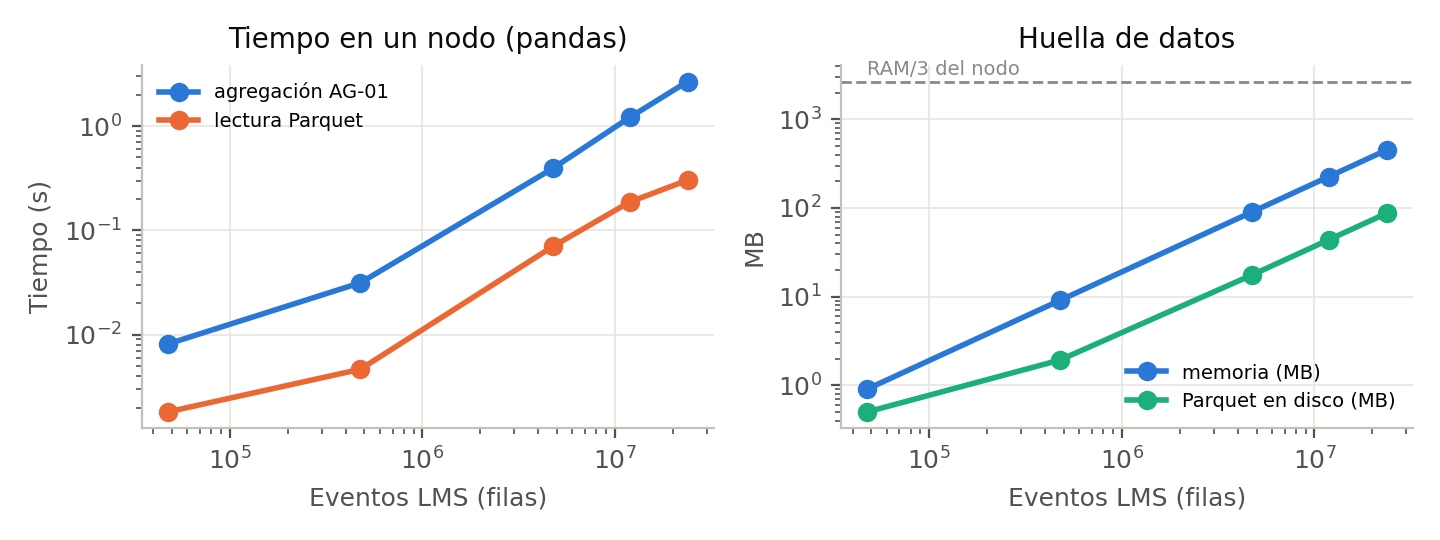
\includegraphics[width=0.92\textwidth]{figuras/fig_escalabilidad.png}
\caption{Tiempo y huella de datos frente al número de eventos (escala log–log).}\label{fig:escala}
\fuente{\texttt{src/benchmark\_escalabilidad.py}.}
\end{figure}

\textbf{Análisis de las cuatro V.}
\begin{itemize}
\item \textbf{Volumen.} El caso real ocupa \benchUciKb{} kB en CSV y \nEvLimpios{} eventos simulados.
Incluso con \benchMaxFilas{} eventos, la huella es de \benchMaxMem{} MB (\benchBpf{} bytes por fila)
y la agregación tarda \benchMaxT{} s. En MongoDB, AG-01 sobre los datos reales tarda \benchMongo{} s.
\item \textbf{Velocidad.} Las notas se actualizan tres veces al año y la decisión (derivar a tutoría) es
por lotes, al cierre de cada período. No hay un requisito de latencia que justifique
\emph{streaming}.
\item \textbf{Variedad.} La heterogeneidad (tabular, documental, texto) se resuelve con el almacenamiento
híbrido, no con cómputo distribuido.
\item \textbf{Costo.} Spark exige JVM, configuración de clúster y serialización, lo que añade complejidad
operativa y puntos de fallo sin mejorar ningún tiempo relevante del caso.
\end{itemize}

\textbf{Umbral de decisión.} Con \benchBpf{} bytes por fila y un margen $\times$3 para intermedios, un
nodo de 8 GB procesa unos \benchMaxNodo{} millones de eventos en memoria. La Tabla~\ref{tab:escenarios}
proyecta escenarios con la tasa del generador (\benchEvMat{} eventos por matrícula y año) y el
rendimiento medido (\benchFps{} millones de filas/s). Estas proyecciones son extrapolaciones lineales
bajo supuestos declarados.

\begin{table}[H]
\centering\small
\caption{Escenarios de escalado (supuestos explícitos; extrapolación del rendimiento medido).}\label{tab:escenarios}
\ajustar{generated/tab_escenarios.tex}
\fuente{\texttt{results/escalabilidad\_escenarios.csv}.}
\end{table}

\textbf{Decisión.} \textbf{No se implementa Spark.} El volumen real está \benchOrdenes{} órdenes de magnitud por debajo del umbral de un nodo, y el benchmark lo confirma. Spark estaría justificado en
el escenario de una red nacional con registros de clics (\emph{clickstream}): unos $10^{9}$--$10^{10}$
eventos al año, que superan la memoria de un nodo, con ingesta continua (Spark Structured Streaming
o Kafka), particionado por centro y fecha en Parquet y agregaciones distribuidas equivalentes a
AG-01. La arquitectura actual ya facilita esa migración: Parquet columnar, agregaciones expresadas
como \texttt{groupby} y un orquestador por etapas. Forzar Spark en este caso no aportaría el “valor
real” que exige la bonificación.

% =============================================================================
\section{Resultados e interpretación}
% =============================================================================
\textbf{Convenciones.} Las secciones 8.1 a 8.4 usan solo datos reales, salvo las columnas marcadas
[SIM]. Los intervalos son al 95\,\%: Wilson para proporciones, $t$ para medias y \emph{bootstrap}
percentil (2.000 réplicas) para tamaños de efecto. Las comparaciones múltiples se corrigen por Holm.
Como 370 estudiantes aportan dos matrículas, las pruebas se estratifican por asignatura y los
modelos logísticos inferenciales usan errores agrupados por estudiante.

\subsection{Descripción de la población}
\begin{table}[H]
\centering\scriptsize
\caption{Descriptivos por asignatura (medianas y rango intercuartílico; notas de evaluados).}\label{tab:descriptivos}
\ajustar{generated/tab_descriptivos.tex}
\fuente{\texttt{results/descriptivos.csv}.}
\end{table}
La prevalencia de reprobación final es el doble en Matemáticas (\prevMat{} \prevIcMat{}) que en
Portugués (\prevPor{} \prevIcPor{}), con intervalos que no se solapan (Tabla~\ref{tab:descriptivos}).
Las faltas son asimétricas (mediana muy inferior al máximo de 75), lo que justifica los métodos no
paramétricos.

\subsection{P1: evolución de la nota y combinaciones centro–asignatura}\label{sec:p1}
\begin{figure}[H]
\centering
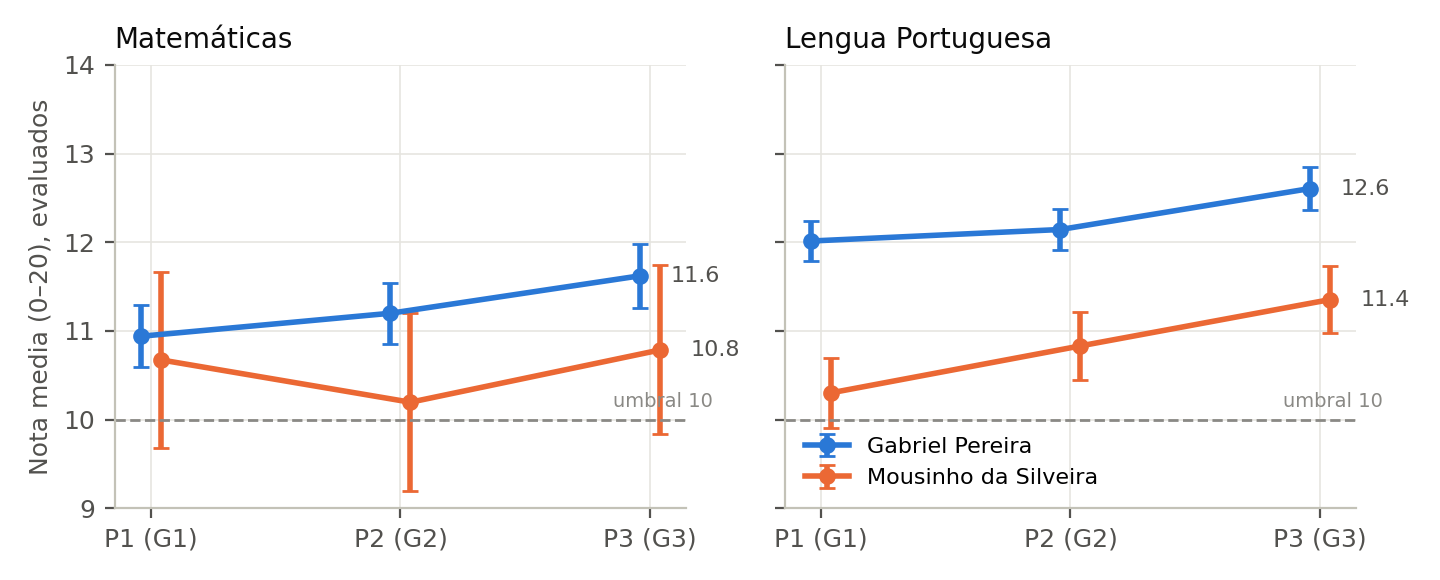
\includegraphics[width=0.95\textwidth]{figuras/fig_p1_evolucion.png}
\caption{Nota media por período, asignatura y escuela (evaluados; IC 95\,\%).}\label{fig:p1evol}
\fuente{\texttt{results/p1\_medias\_periodo\_escuela.csv}.}
\end{figure}

\begin{table}[H]
\centering\small
\caption{P1: cambio de la nota entre períodos (matrículas evaluadas en los tres períodos; Wilcoxon con Holm).}\label{tab:p1pruebas}
\ajustar{generated/tab_p1_pruebas.tex}
\fuente{\texttt{results/p1\_pruebas\_evolucion.csv}. $r_{rb}$: correlación biserial de rangos para muestras pareadas.}
\end{table}

\textbf{Evolución.} La nota media aumenta ligeramente a lo largo del curso en ambas asignaturas
(Figura~\ref{fig:p1evol}, Tabla~\ref{tab:p1pruebas}). En Portugués el cambio es sistemático
(Friedman $\chi^2$ = \friedChiPor{}, $p$ \friedPPor{}; W de Kendall = \kendallWPor{}), con una
mejora media de P1 a P3 de \difPUnoTresPor{} puntos \difPUnoTresIcPor{}. En Matemáticas es menor y
de magnitud despreciable ($\chi^2$ = \friedChiMat{}, $p$ = \friedPMat{}; W = \kendallWMat{};
P1$\rightarrow$P3 = \difPUnoTresMat{} \difPUnoTresIcMat{}). En la práctica, ningún cambio altera la
situación de aprobación de un estudiante típico (menos de un punto sobre 20). \textbf{Advertencia de
interpretación:} el aumento se calcula sobre quienes siguen evaluados. Los que abandonan salen de la
media (sesgo de supervivencia), y si se incluyeran sus ceros la media de Matemáticas
\emph{descendería} de \mediaCerosMatPUno{} en P1 a \mediaCerosMatPTres{} en P3. Este contraste
justifica la regla R-08.

\begin{figure}[H]
\centering
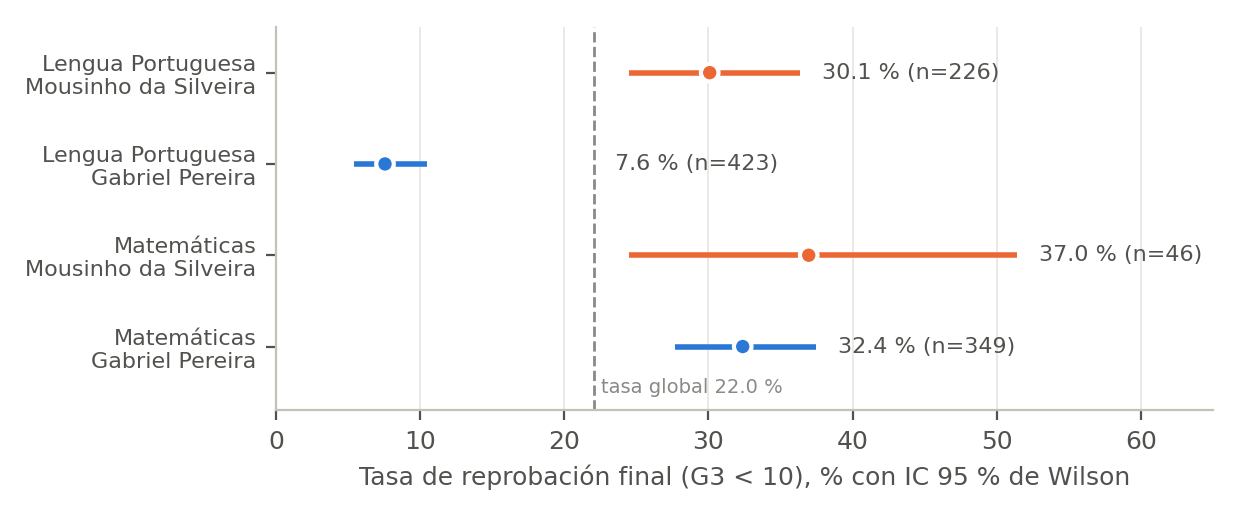
\includegraphics[width=0.8\textwidth]{figuras/fig_p1_reprobacion.png}
\caption{Tasa de reprobación final por asignatura y escuela (IC 95\,\% de Wilson).}\label{fig:p1rep}
\fuente{\texttt{results/p1\_reprobacion\_escuela\_asignatura.csv}.}
\end{figure}

\begin{table}[H]
\centering\small
\begin{minipage}[t]{0.56\textwidth}\centering
\caption{Reprobación por asignatura y escuela.}\label{tab:p1rep}
\ajustar{generated/tab_p1_reprobacion.tex}
\end{minipage}\hfill
\begin{minipage}[t]{0.42\textwidth}\centering
\caption{Reprobación en P3 según el estado en P1.}\label{tab:persist}
\ajustar{generated/tab_p1_persistencia.tex}
\end{minipage}
\fuente{\texttt{results/p1\_reprobacion\_escuela\_asignatura.csv} y \texttt{results/p1\_persistencia.csv}. “Prioritaria”: límite inferior del IC mayor que la tasa global (\prevTot{}).}
\end{table}

\textbf{Combinaciones que exigen intervención.} Se definió como prioritaria una combinación cuyo
límite inferior del IC de Wilson supera la tasa global. Tres de las cuatro cumplen el criterio
(Tabla~\ref{tab:p1rep}, Figura~\ref{fig:p1rep}):
\begin{itemize}
\item Matemáticas en ambos centros: GP con \tasaMatGp{} \tasaIcMatGp{} y MS con \tasaMatMs{}
\tasaIcMatMs{}. La diferencia entre centros no es significativa ($\chi^2$ = \chiEscMat{}, $p$ Holm
= \chiEscPMat{}, V = \vEscMat{}).
\item Portugués en Mousinho da Silveira: \tasaPorMs{} \tasaIcPorMs{} frente a \tasaPorGp{} en
Gabriel Pereira. La diferencia de \difEscPor{} puntos porcentuales es significativa y de tamaño
moderado ($\chi^2$ = \chiEscPor{}, $p$ Holm \chiEscPPor{}, V = \vEscPor{}).
\end{itemize}
El efecto de centro es, por tanto, específico de la asignatura. En los datos disponibles, la
diferencia en Portugués no puede separarse de la composición del alumnado de cada centro (dato
observacional). Además, la reprobación en P1 anticipa con fuerza la final
(Tabla~\ref{tab:persist}): reprueban al final el \persMatRep{} de quienes reprueban P1 en Matemáticas
frente al \persMatApr{} de quienes lo aprueban, y en Portugués el \persPorRep{} frente al
\persPorApr{}. Este hallazgo fundamenta el corte temprano.

\subsection{P2: condiciones que distinguen el rendimiento sobre y bajo el promedio}\label{sec:p2}
Se compararon las matrículas evaluadas con $G3$ por encima de la media de su asignatura con las que
quedaron por debajo: \nSobreMat{} frente a \nBajoMat{} en Matemáticas y \nSobrePor{} frente a
\nBajoPor{} en Portugués (Tabla~\ref{tab:p2}, Figura~\ref{fig:p2}).

\begin{table}[H]
\centering\scriptsize
\caption{P2: comparación sobre/bajo el promedio por asignatura (MW: Mann-Whitney U con $\delta$ de Cliff; $\chi^2$: chi-cuadrado con diferencia de proporciones y V de Cramér; $p$ corregido por Holm).}\label{tab:p2}
\ajustar{generated/tab_p2.tex}
\fuente{\texttt{results/p2\_condiciones.csv}. Resumen: mediana [RIC] o porcentaje. [SIM] = variable simulada.}
\end{table}

\begin{figure}[H]
\centering
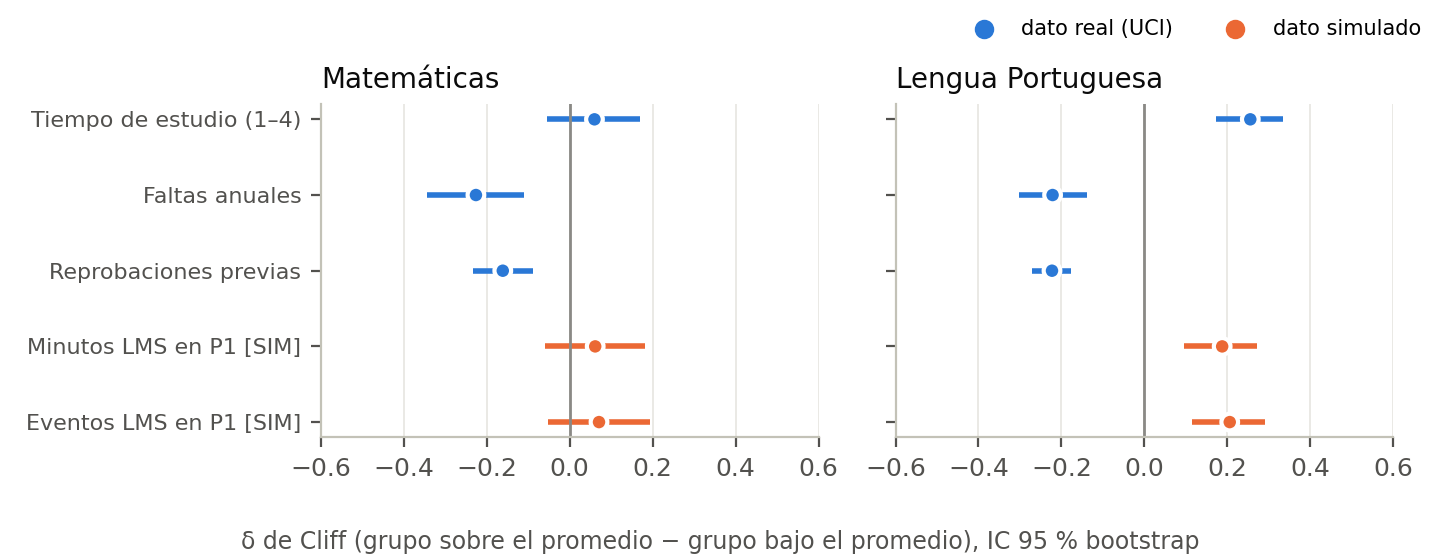
\includegraphics[width=0.95\textwidth]{figuras/fig_p2_cliff.png}
\caption{Tamaño de efecto ($\delta$ de Cliff, IC 95\,\% \emph{bootstrap}) de las variables ordinales y numéricas en P2.}\label{fig:p2}
\fuente{\texttt{results/p2\_condiciones.csv}.}
\end{figure}

\textbf{Interpretación (datos reales).}
\begin{itemize}
\item En ambas asignaturas, quienes quedan bajo el promedio tienen \textbf{más faltas}
($\delta$ = \cdMatFaltas{} en MAT; \cdPorFaltas{} en POR) y \textbf{más reprobaciones previas}
($\delta$ = \cdMatReprobacionesPrevias{} y \cdPorReprobacionesPrevias{}). Son efectos pequeños pero
consistentes.
\item El \textbf{tiempo de estudio} distingue en Portugués ($\delta$ = \cdPorTiempoEstudio{}), no en
Matemáticas ($\delta$ = \cdMatTiempoEstudio{}).
\item La aspiración a educación superior es mucho más frecuente sobre el promedio en Portugués
(V = \cdPorDeseaSuperior{}).
\item El \textbf{refuerzo escolar} es \emph{más} frecuente en el grupo bajo el promedio (V =
\cdMatApoyoEscolar{} en MAT). Esto refleja que el refuerzo se asigna a quien ya tiene dificultades
(causalidad inversa), no que perjudique. Es un ejemplo de por qué la asociación no implica
causalidad.
\item Las clases pagadas no distinguen.
\end{itemize}
\textbf{Variables simuladas.} Los minutos LMS\SIM{} muestran $\delta$ = \cdPorSimLmsMinutosPUno{} en
Portugués y \cdMatSimLmsMinutosPUno{} en Matemáticas. No es un hallazgo: el generador hace depender
el LMS del tiempo de estudio y de la aspiración a estudios superiores, que en Portugués sí se
asocian al rendimiento. La señal simulada solo reproduce, atenuada, la de esas covariables reales.

\subsection{Pregunta principal: combinación de factores y acompañamiento asociado}\label{sec:principal}
Se definieron tres factores: \emph{alta inasistencia} (cuartil superior de faltas de la asignatura;
real), \emph{reprobaciones previas} (1 o más; real) y \emph{bajo involucramiento LMS} (cuartil
inferior de minutos LMS en P1; simulado). Conforme a R-09, el análisis usa las \nConfiables{}
matrículas con faltas confiables.

\begin{table}[H]
\centering\scriptsize
\caption{Perfiles de riesgo: reprobación final y acompañamiento asociado (columnas [SIM] simuladas).}\label{tab:perfiles}
\ajustar{generated/tab_principal_perfiles.tex}
\fuente{\texttt{results/principal\_perfiles.csv}; matrículas con faltas confiables.}
\end{table}

\begin{figure}[H]
\centering
\begin{minipage}[c]{0.5\textwidth}\centering
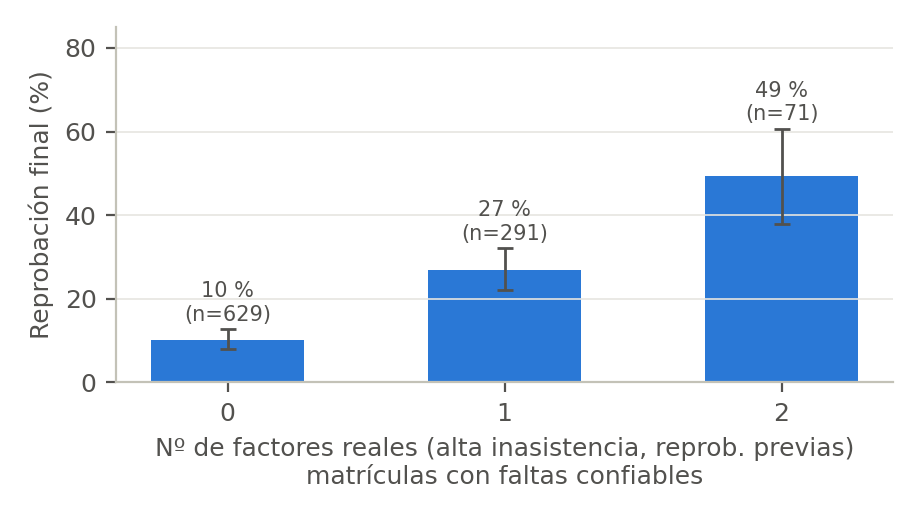
\includegraphics[width=\linewidth]{figuras/fig_principal_factores.png}
\end{minipage}\hfill
\begin{minipage}[c]{0.47\textwidth}\centering\scriptsize
\ajustar{generated/tab_principal_or.tex}
\end{minipage}
\caption{Gradiente de reprobación según el número de factores reales (izquierda) y odds ratios ajustados con errores agrupados por estudiante (derecha).}\label{fig:principal}
\fuente{\texttt{results/principal\_gradiente.csv} y \texttt{results/principal\_or.csv}.}
\end{figure}

\textbf{Interpretación.} La reprobación crece de forma monótona con el número de factores reales:
\gradCero{} \gradIcCero{} sin factores (n = \gradNCero{}), \gradUno{} \gradIcUno{} con uno
(n = \gradNUno{}) y \gradDos{} \gradIcDos{} con ambos (n = \gradNDos{}) (Figura~\ref{fig:principal}).
Ajustando por asignatura, las reprobaciones previas multiplican las odds por \orReprob{}
\orReprobIc{} y la alta inasistencia por \orInasist{} \orInasistIc{}. La regla R-09 importa: si se
incluyen los no evaluados con 0 faltas no confiables, el OR de inasistencia se atenúa a
\orInasistTodas{} \orInasistTodasIc{} y deja de ser significativo, lo que llevaría a una conclusión
errónea. En la Tabla~\ref{tab:perfiles}, los perfiles con reprobaciones previas tienen tasas de reprobación de entre \perfRepMin{} y \perfRepMax{}, con independencia del LMS. El factor LMS\SIM{} no muestra un patrón propio,
consistente con su proceso generador. En cuanto al acompañamiento\SIM{}, los perfiles de mayor
riesgo concentran más alertas y tutorías, porque la regla simulada las dispara con $G1<10$. AG-04 muestra que el \agCuatroMedio{} de las alertas de nivel medio y el \agCuatroAlto{} de las de nivel alto tienen una tutoría posterior, y que ninguna de nivel bajo la tiene. Esto demuestra la capacidad del pipeline para
responder este tipo de consulta, pero no mide la eficacia de las tutorías.

\subsection{Modelo de predicción temprana}\label{sec:modelo}
\textbf{Diseño.} Se definieron escenarios de información creciente: C, solo antecedentes al
matricular (sin notas); \textbf{A, corte P1}, que es C más $G1$ y es el escenario principal; y B,
corte P2, que añade $G2$. Se comparan una línea base (probabilidad a priori), una regresión
logística (interpretable) y dos modelos no lineales: \emph{random forest} (Breiman, 2001) y
\emph{gradient boosting} (Friedman, 2001). La evaluación usa validación cruzada estratificada y
agrupada por estudiante (5 pliegues) en entrenamiento, y una evaluación final única en el conjunto
de prueba reservado (\nTest{} matrículas, \nRiesgoTest{} en riesgo, \prevTest{}). Por el
desbalance, se reportan AUC-PR, recall, precisión, F1 y Brier además del AUC-ROC (Saito \&
Rehmsmeier, 2015). El umbral de decisión se fijó en entrenamiento, con predicciones fuera de pliegue,
como el mayor umbral que logra un recall de al menos 0,80, porque en alerta temprana omitir a un
estudiante en riesgo cuesta más que una derivación innecesaria.

\begin{sidewaystable}
\centering\scriptsize
\caption{Métricas de los modelos por escenario (CV: media $\pm$ DE en 5 pliegues agrupados; test: conjunto reservado, IC 95\,\% \emph{bootstrap} por estudiante).}\label{tab:modelos}
\begin{tabular}{llllllllll}
\toprule
Escenario & Modelo & AUC-ROC CV & AUC-PR CV & AUC-ROC test [IC 95\,\%] & AUC-PR & Recall & Precisión & F1 & Brier \\
\midrule
A: corte P1 (principal) & Línea base (prior) & 0,500 $\pm$ 0,000 & 0,215 & 0,500 [0,500; 0,500] & 0,241 & 0,000 & 0,000 & 0,000 & 0,183 \\
A: corte P1 (principal) & Regresión logística & 0,924 $\pm$ 0,011 & 0,762 & 0,948 [0,918; 0,972] & 0,853 & 0,902 & 0,667 & 0,767 & 0,080 \\
A: corte P1 (principal) & Random forest & 0,921 $\pm$ 0,018 & 0,739 & 0,940 [0,904; 0,969] & 0,845 & 0,882 & 0,714 & 0,789 & 0,097 \\
A: corte P1 (principal) & Gradient boosting & 0,925 $\pm$ 0,007 & 0,761 & 0,944 [0,915; 0,968] & 0,830 & 0,922 & 0,671 & 0,777 & 0,083 \\
C: sin notas & Regresión logística & 0,775 $\pm$ 0,029 & 0,481 & 0,738 [0,664; 0,804] & 0,532 & 0,686 & 0,376 & 0,486 & 0,158 \\
C: sin notas & Random forest & 0,799 $\pm$ 0,048 & 0,508 & 0,750 [0,676; 0,817] & 0,563 & 0,667 & 0,378 & 0,482 & 0,154 \\
C: sin notas & Gradient boosting & 0,785 $\pm$ 0,030 & 0,490 & 0,762 [0,689; 0,824] & 0,557 & 0,745 & 0,358 & 0,484 & 0,153 \\
C + LMS [SIM] & Regresión logística & 0,774 $\pm$ 0,022 & 0,480 & 0,737 [0,660; 0,805] & 0,520 & 0,667 & 0,366 & 0,472 & 0,159 \\
C + LMS [SIM] & Random forest & 0,800 $\pm$ 0,026 & 0,521 & 0,755 [0,674; 0,829] & 0,553 & 0,745 & 0,380 & 0,503 & 0,153 \\
C + LMS [SIM] & Gradient boosting & 0,777 $\pm$ 0,028 & 0,462 & 0,777 [0,707; 0,839] & 0,575 & 0,784 & 0,381 & 0,513 & 0,148 \\
A + LMS [SIM] & Regresión logística & 0,923 $\pm$ 0,010 & 0,746 & 0,949 [0,919; 0,972] & 0,853 & 0,902 & 0,657 & 0,760 & 0,081 \\
A + LMS [SIM] & Random forest & 0,921 $\pm$ 0,016 & 0,750 & 0,945 [0,911; 0,973] & 0,864 & 0,882 & 0,682 & 0,769 & 0,096 \\
A + LMS [SIM] & Gradient boosting & 0,921 $\pm$ 0,007 & 0,745 & 0,948 [0,920; 0,972] & 0,846 & 0,902 & 0,657 & 0,760 & 0,080 \\
A + faltas anuales & Regresión logística & 0,925 $\pm$ 0,011 & 0,766 & 0,945 [0,912; 0,970] & 0,847 & 0,882 & 0,692 & 0,776 & 0,080 \\
A + faltas anuales & Random forest & 0,923 $\pm$ 0,017 & 0,753 & 0,942 [0,906; 0,971] & 0,860 & 0,882 & 0,726 & 0,796 & 0,094 \\
A + faltas anuales & Gradient boosting & 0,925 $\pm$ 0,020 & 0,751 & 0,953 [0,927; 0,975] & 0,855 & 0,882 & 0,714 & 0,789 & 0,077 \\
B: corte P2 & Regresión logística & 0,962 $\pm$ 0,016 & 0,892 & 0,984 [0,969; 0,995] & 0,958 & 0,902 & 0,836 & 0,868 & 0,044 \\
B: corte P2 & Random forest & 0,962 $\pm$ 0,012 & 0,880 & 0,988 [0,975; 0,996] & 0,965 & 0,882 & 0,882 & 0,882 & 0,055 \\
B: corte P2 & Gradient boosting & 0,962 $\pm$ 0,018 & 0,890 & 0,984 [0,968; 0,996] & 0,960 & 0,902 & 0,885 & 0,893 & 0,041 \\
\bottomrule
\end{tabular}

\fuente{\texttt{results/modelo\_metricas.csv}. Recall, precisión y F1 con el umbral fijado en entrenamiento (recall OOF $\geq$ 0,80).}
\end{sidewaystable}

\begin{figure}[H]
\centering
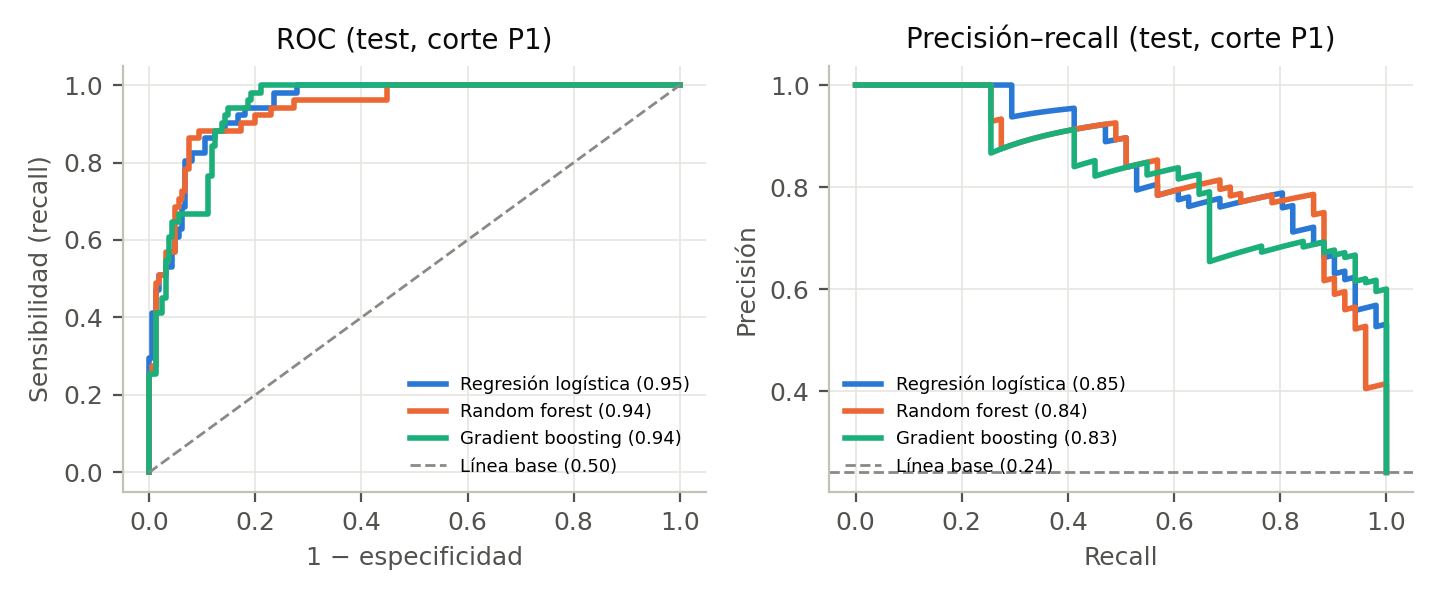
\includegraphics[width=0.95\textwidth]{figuras/fig_modelo_roc_pr.png}
\caption{Curvas ROC y precisión–recall en prueba, escenario A (corte P1).}\label{fig:roc}
\fuente{\texttt{src/analysis.py::modelado}.}
\end{figure}

\textbf{Resultados.} La Tabla~\ref{tab:modelos} reúne las métricas de todos los escenarios y modelos, y la Figura~\ref{fig:roc} muestra las curvas del escenario principal. En el escenario A, la regresión logística obtiene un AUC-ROC en prueba
de \aucALr{} \aucIcALr{} (CV: \cvaucALr{}), un AUC-PR de \aucprALr{} (línea base: \aucprABase{}) y,
con el umbral preespecificado, recall \recALr{}, precisión \precALr{}, especificidad \espALr{}, F1
\foneALr{} y Brier \brierALr{} (línea base: \brierABase{}). La matriz de confusión en prueba es
VP = \tpALr{}, FN = \fnALr{}, FP = \fpALr{} y VN = \tnALr{}: se detectan \tpALr{} de los \nRiesgoTest{} casos en riesgo, a costa de \fpALr{} derivaciones innecesarias. Los modelos no lineales no superan a la logística
(\emph{random forest} \aucARf{}, \emph{gradient boosting} \aucAGb{}), así que se prefiere el modelo
interpretable. El valor de la información temprana es claro: pasar de C (sin notas, AUC \aucCLr{})
a A (con $G1$) añade $\Delta$AUC = \dACLr{} \dIcACLr{}. Esperar a P2 añade solo \dBALr{}
\dIcBALr{} más, y a cambio se pierde un período de intervención. El rendimiento es similar por
centro y asignatura (Tabla~\ref{tab:estratos}), sin degradación en el centro minoritario.

\begin{figure}[H]
\centering
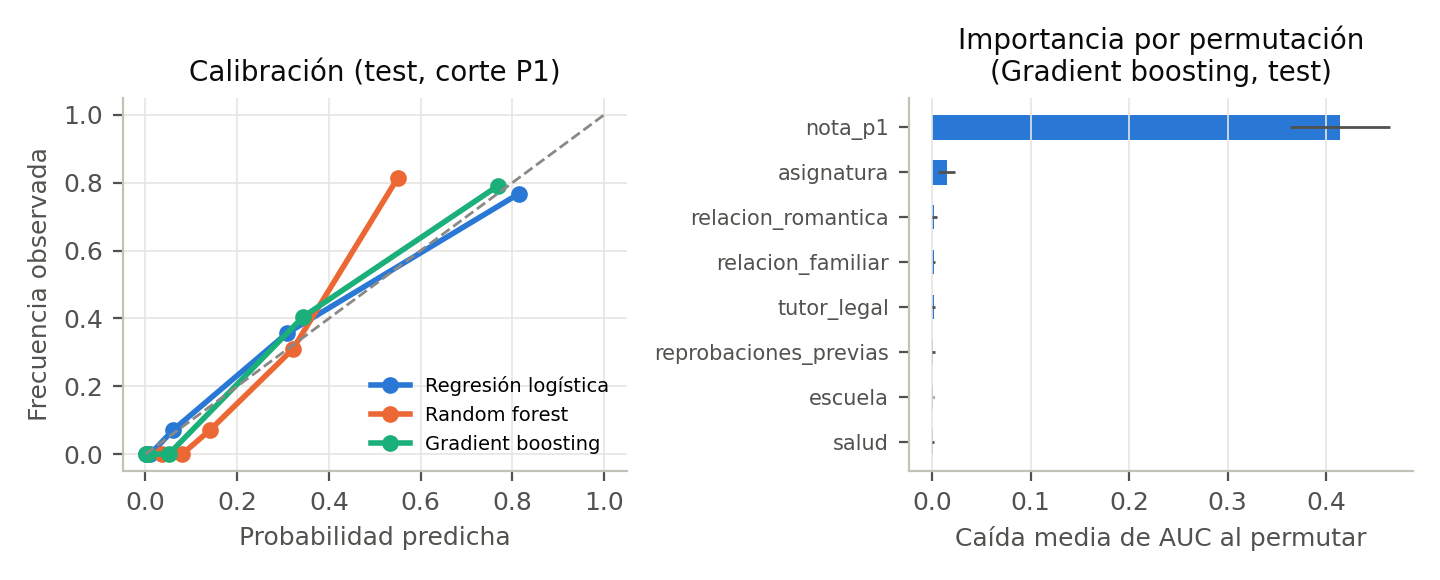
\includegraphics[width=0.95\textwidth]{figuras/fig_modelo_calibracion_importancia.png}
\caption{Calibración en prueba (izquierda) e importancia por permutación del mejor modelo no lineal en CV (derecha), escenario A.}\label{fig:calib}
\fuente{\texttt{results/modelo\_importancia\_permutacion.csv}.}
\end{figure}

\begin{table}[H]
\centering\small
\begin{minipage}[t]{0.52\textwidth}\centering
\caption{Odds ratios del modelo logístico parsimonioso (corte P1; entrenamiento; errores agrupados por estudiante).}\label{tab:odds}
\ajustar{generated/tab_odds.tex}
\end{minipage}\hfill
\begin{minipage}[t]{0.45\textwidth}\centering
\caption{Desempeño del modelo A (logística) por estrato en prueba.}\label{tab:estratos}
\ajustar{generated/tab_estratos.tex}
\end{minipage}
\fuente{\texttt{results/modelo\_odds\_ratios.csv} y \texttt{results/modelo\_estratos.csv}. Predictores del modelo parsimonioso preespecificados.}
\end{table}

\textbf{Interpretación.} Cada punto adicional en $G1$ multiplica las odds de reprobar por
\orNotaUno{} \orNotaUnoIc{}, es decir, las reduce en torno al \orNotaUnoRed{} por punto (Tabla~\ref{tab:odds}). Condicionado a $G1$,
cursar Portugués reduce las odds (OR \orPor{} \orPorIc{}), igual que aspirar a educación superior
(OR \orSup{} \orSupIc{}). Las reprobaciones previas y el centro dejan de ser significativos una vez
que se conoce $G1$ (centro MS: OR \orEsc{} \orEscIc{}), porque su efecto ya está incorporado en esa
nota. La importancia por permutación coincide con esta lectura: permutar $G1$ reduce el AUC en
\impNotaUno{}, y la siguiente variable (\impSegunda{}) solo en \impSegundaV{}. La calibración de la
logística es aceptable (Figura~\ref{fig:calib}); el \emph{random forest} subestima las
probabilidades altas. Por eso, para comunicar probabilidades se recomienda la logística.

\subsection{Sensibilidad: datos reales frente a datos simulados}\label{sec:sens}
\begin{table}[H]
\centering\small
\caption{Análisis de sensibilidad: cambio de AUC-ROC en prueba al añadir o quitar información (IC 95\,\% \emph{bootstrap} pareado por estudiante).}\label{tab:sens}
\ajustar{generated/tab_sensibilidad.tex}
\fuente{\texttt{results/modelo\_sensibilidad.csv}.}
\end{table}

\begin{itemize}
\item \textbf{Con y sin variables simuladas.} Añadir las cuatro variables LMS\SIM{} del corte P1 no
cambia el desempeño: $\Delta$AUC = \dAsimALr{} \dIcAsimALr{} en A y \dCsimCLr{} \dIcCsimCLr{} en C
(logística). Todos los intervalos incluyen el cero en los tres algoritmos (Tabla~\ref{tab:sens}).
Es el resultado esperado de un generador no circular: el LMS simulado no contiene información sobre
$G3$ más allá de las covariables reales que ya están en el modelo.
\item \textbf{Contrafactual didáctico de circularidad.} Si el LMS se hubiera generado “correlacionado
con el riesgo real”, como proponía el avance (aquí, $\text{minutos} \propto e^{0{,}15\,G3}$), el
escenario C pasaría de AUC \circCHonesto{} a \circCMasCircular{}. Sería una mejora ficticia de \circDifC{}, producida solo por la construcción de los datos. Esta cifra cuantifica el riesgo que motivó
el rediseño del generador.
\item \textbf{Faltas anuales.} Añadirlas al modelo temprano no mejora el AUC (\dAfalALr{}
\dIcAfalALr{}). Por tanto, excluirlas por fuga temporal (L-02) no tiene costo.
\end{itemize}
\textbf{Separación de hallazgos.} Todos los hallazgos sustantivos (§\ref{sec:p1}, §\ref{sec:p2}, §\ref{sec:principal} en sus factores reales y §\ref{sec:modelo}) provienen de datos reales. Las cifras sobre LMS, tutorías, alertas y texto
son demostraciones de que el pipeline integra, valida y consulta evidencia heterogénea.

\subsection{Componente no estructurado: texto libre de las alertas}\label{sec:texto}
Las \nNotasTexto{} notas de orientación\SIM{} se normalizaron (minúsculas, expansión de
abreviaturas como “est.” $\rightarrow$ “estudiante”, eliminación de tildes, puntuación y espacios
repetidos), se tokenizaron sin palabras vacías y se categorizaron por léxico en académico,
asistencia, familiar, conducta y motivación (\texttt{transform\_synthetic.py::categorizar}). Los
resultados se guardan en el propio documento (\texttt{texto\_normalizado}, \texttt{categoria}),
se indexan con un índice de texto en español y se agregan con AG-06 (Tabla~\ref{tab:ag06}). La Tabla~\ref{tab:texto} muestra ejemplos de la normalización y la Tabla~\ref{tab:terminos} (Anexo~F) los términos más frecuentes. La
exactitud frente a la categoría verdadera del generador es \exactitudTexto{}. \textbf{Este valor no
mide la capacidad de generalizar}: el léxico se construyó conociendo las plantillas del generador,
por lo que solo demuestra que la transformación está bien implementada. Con notas reales se
necesitaría una muestra etiquetada por orientadores y un clasificador supervisado evaluado en datos
no vistos.

\begin{table}[H]
\centering\scriptsize
\begin{minipage}[t]{0.46\textwidth}\centering
\caption{AG-06\SIM: categoría inferida $\times$ nivel de alerta.}\label{tab:ag06}
\ajustar{generated/tab_mongo_ag06.tex}
\end{minipage}\hfill
\begin{minipage}[t]{0.5\textwidth}\centering
\caption{Ejemplos de normalización\SIM.}\label{tab:texto}
\ajustar{generated/tab_texto_ejemplos.tex}
\end{minipage}
\fuente{\texttt{results/mongo\_AG-06.csv} y \texttt{results/texto\_ejemplos.csv}. Datos simulados.}
\end{table}

\subsection{Utilidad y limitaciones de los resultados}
\textbf{Utilidad.} Al cierre de P1, una regla basada en el modelo A identificaría al \recALr{} de los estudiantes que reprobarán (recall), y el \precALr{} de las derivaciones serían correctas (precisión). Es un criterio operativo y
explicable para orientar tutorías.

\textbf{Limitaciones.}
\begin{enumerate}[label=(\roman*)]
\item Los datos son \emph{observacionales}: ninguna asociación es causal.
\item La población es de dos centros portugueses en 2005--2006; la validez externa es limitada.
\item $G1$ domina la predicción; el modelo no identifica a quien reprobará pese a aprobar P1 (\persMatApr{} en MAT).
\item Las fuentes F2 y F3 son simuladas: su utilidad predictiva real está por demostrar.
\item El conjunto de prueba es pequeño (\nTest{} matrículas), de ahí la anchura de los IC.
\item La identidad tiene \nFalsosNeg{} posibles falsos negativos.
\item El umbral de recall 0,80 es una decisión de política que debería fijar la institución según su capacidad de tutoría.
\end{enumerate}

% =============================================================================
\section{Conclusiones y recomendaciones}
% =============================================================================
\subsection{Conclusiones}
\begin{enumerate}
\item \textbf{Arquitectura.} El almacenamiento híbrido es coherente con el problema. PostgreSQL en 3FN
garantiza la integridad del registro académico: \nControlesOk{} de \nControlesSql{} controles
superados. MongoDB, con validadores \texttt{\$jsonSchema} y \texttt{\$expr}, modela la evidencia
anidada y variable con cobertura total. Parquet sirve de contrato con la capa analítica.
\item \textbf{Calidad.} Los principales problemas del registro UCI eran semánticos: identidad, notas 0
y faltas no confiables. La regla de identidad en dos etapas corrigió las cifras del avance a
\nEst{} estudiantes, \nMat{} matrículas y \nCal{} calificaciones, y recuperó 16 matrículas reales
que se habían perdido. Las reglas sobre datos simulados detectaron exactamente los defectos
inyectados.
\item \textbf{P1.} La reprobación se concentra en Matemáticas (ambos centros) y en Portugués en
Mousinho da Silveira (\tasaPorMs{}). La nota media apenas varía a lo largo del curso cuando se
excluyen los abandonos.
\item \textbf{P2 y pregunta principal.} Las reprobaciones previas y la inasistencia distinguen el bajo
rendimiento y se acumulan: la reprobación pasa de \gradCero{} sin factores a \gradDos{} con ambos.
\item \textbf{Predicción temprana.} Con información del primer período, sin $G3$, sin faltas anuales y
sin compartir estudiantes entre entrenamiento y prueba, un modelo logístico interpretable alcanza un
AUC de \aucALr{} y un recall de \recALr{}. La nota $G1$ aporta casi toda la señal.
\item \textbf{Datos simulados.} No aportan información predictiva ($\Delta$AUC = \dAsimALr{}), como
exige un generador no circular. El contrafactual muestra que un generador circular habría fabricado
una mejora de \circDifC{} en el AUC.
\item \textbf{Escalabilidad.} Spark no está justificado. El benchmark procesa \benchMaxFilas{} eventos
en \benchMaxT{} s en un solo nodo, y el caso real está \benchOrdenes{} órdenes de magnitud por debajo de ese umbral.
\end{enumerate}

\subsection{Recomendaciones para la coordinación y la orientación}
\begin{itemize}
\item Institucionalizar una \textbf{alerta al cierre del primer período}: toda matrícula con $G1<10$ o
con probabilidad del modelo A superior al umbral se deriva a tutoría antes de enero.
\item Priorizar \textbf{Matemáticas} en ambos centros y \textbf{Portugués en Mousinho da Silveira}.
\item Dar seguimiento específico a los estudiantes con \textbf{reprobaciones previas} desde la
matrícula (escenario C), antes incluso de la primera nota.
\item Registrar la asistencia por período, no solo anual, y codificar explícitamente los abandonos, en
lugar de registrar notas 0 con 0 faltas.
\end{itemize}

\subsection{Mejoras y próximos pasos}
\begin{enumerate}
\item Sustituir F2 y F3 por exportaciones reales del LMS y del departamento de orientación, reutilizando validadores y reglas, y repetir la sensibilidad.
\item Evaluar el efecto de las tutorías con un diseño cuasiexperimental (p. ej., regresión discontinua en el umbral $G1 = 10$).
\item Validar el modelo en una cohorte posterior (validación temporal) y recalibrarlo por centro.
\item Añadir un clasificador supervisado de texto entrenado con notas etiquetadas.
\item Orquestar el pipeline con un planificador (p. ej., Airflow) y publicar el tablero de alertas desde la colección \texttt{alertas\_riesgo}.
\end{enumerate}

% =============================================================================
\section{Evidencias técnicas}
% =============================================================================
La Tabla~\ref{tab:repo} describe la estructura del repositorio.

\textbf{Repositorio:} \repourl{}\\
\textbf{Copia adjunta:} \repozip{}. Contiene la estructura completa de la Tabla~\ref{tab:repo}: datos, código, consultas, resultados, registros de ejecución y la fuente de este informe. Se reproduce con las instrucciones siguientes.

\begin{table}[H]
\centering\scriptsize
\caption{Estructura del repositorio y artefactos entregados.}\label{tab:repo}
\begin{tabular}{>{\raggedright\arraybackslash}p{4.3cm}>{\raggedright\arraybackslash}p{10.8cm}}
\toprule
Ruta & Contenido \\
\midrule
\texttt{run\_pipeline.py} & Punto de entrada único (etapas 1–11). \\
\texttt{docker-compose.yml}, \texttt{.env.example} & PostgreSQL 16 y MongoDB 8; variables de conexión sin secretos. \\
\texttt{requirements.txt}, \texttt{requirements-lock.txt} & Versiones fijadas y entorno congelado. \\
\texttt{data/raw/} & \texttt{student-mat.csv}, \texttt{student-por.csv} (UCI) y \texttt{synthetic/} (JSON crudos + verdad del generador). \\
\texttt{data/staging/} & Tablas 3FN, evidencia de identidad, documentos Mongo, cuarentena. \\
\texttt{data/processed/} & \texttt{dataset\_analitico.parquet} (+ \texttt{.csv}), \texttt{diccionario\_datos.csv}, \texttt{linaje.csv}, \texttt{mapeo\_avance\_final.csv}. \\
\texttt{sql/} & \texttt{01\_ddl.sql}, \texttt{02\_vistas\_seguridad.sql}, \texttt{03\_integridad.sql}, \texttt{04\_analiticas.sql}. \\
\texttt{mongo/} & \texttt{validadores.json}, \texttt{indices.json}, \texttt{pipelines.json} (ejecutables también desde \texttt{mongosh}). \\
\texttt{src/} & \texttt{config}, \texttt{tracking}, \texttt{extract}, \texttt{transform}, \texttt{generate\_synthetic}, \texttt{transform\_synthetic}, \texttt{load}, \texttt{integrate}, \texttt{analysis}, \texttt{benchmark\_escalabilidad}, \texttt{report\_tables}. \\
\texttt{tests/test\_pipeline.py} & 17 pruebas \texttt{pytest}. \\
\texttt{notebooks/analisis.ipynb} & Notebook ejecutado: consultas SQL y pipelines Mongo en vivo, reproducción del AUC principal. \\
\texttt{results/}, \texttt{logs/} & Salidas de consultas, pruebas y modelos; conteos por etapa, reglas y checksums. \\
\texttt{informe/} & \texttt{main.tex}, \texttt{generated/} (tablas y macros), \texttt{figuras/}, PDF final. \\
\bottomrule
\end{tabular}
\end{table}

\textbf{Instrucciones de ejecución.}
\begin{lstlisting}[language=bash]
cp .env.example .env && docker compose up -d --wait        # PostgreSQL 16 + MongoDB 8
python3 -m venv .venv && .venv/bin/pip install -r requirements.txt
.venv/bin/python run_pipeline.py --informe                  # pipeline completo + PDF (~90 s)
.venv/bin/python -m pytest -q                               # 17 pruebas
\end{lstlisting}

\textbf{Datos de ejemplo.} El Listado~\ref{lst:ejemplo} muestra un documento real de la colección
\texttt{seguimiento\_riesgo} tras la carga, recortado a dos eventos. El Anexo~F reproduce una alerta
con su historial y sus notas.

\lstinputlisting[caption={Documento de \texttt{seguimiento\_riesgo}\SIM{} (estudiante 1, período P1; recortado a dos eventos; generado desde \texttt{results/mongo\_documentos\_ejemplo.json}).}, label=lst:ejemplo]{generated/ejemplo_seguimiento.json}

% =============================================================================
\section*{Referencias}
\addcontentsline{toc}{section}{Referencias}
% =============================================================================
\begingroup
\setlength{\parindent}{-1.27cm}\setlength{\leftskip}{1.27cm}\setlength{\parskip}{0.35em}\small

Apache Software Foundation. (2024). \emph{Apache Parquet documentation}. \url{https://parquet.apache.org/docs/}

Breiman, L. (2001). Random forests. \emph{Machine Learning, 45}(1), 5–32. \url{https://doi.org/10.1023/A:1010933404324}

Cliff, N. (1993). Dominance statistics: Ordinal analyses to answer ordinal questions. \emph{Psychological Bulletin, 114}(3), 494–509. \url{https://doi.org/10.1037/0033-2909.114.3.494}

Cortez, P. (2008). \emph{Student performance} [Conjunto de datos]. UCI Machine Learning Repository. \url{https://doi.org/10.24432/C5TG7T}

Cortez, P., \& Silva, A. M. G. (2008). Using data mining to predict secondary school student performance. En A. Brito \& J. Teixeira (Eds.), \emph{Proceedings of 5th Future Business Technology Conference (FUBUTEC 2008)} (pp. 5–12). EUROSIS-ETI.

Elmasri, R., \& Navathe, S. B. (2016). \emph{Fundamentals of database systems} (7.ª ed.). Pearson.

Friedman, J. H. (2001). Greedy function approximation: A gradient boosting machine. \emph{The Annals of Statistics, 29}(5), 1189–1232. \url{https://doi.org/10.1214/aos/1013203451}

Holm, S. (1979). A simple sequentially rejective multiple test procedure. \emph{Scandinavian Journal of Statistics, 6}(2), 65–70.

Kaufman, S., Rosset, S., Perlich, C., \& Stitelman, O. (2012). Leakage in data mining: Formulation, detection, and avoidance. \emph{ACM Transactions on Knowledge Discovery from Data, 6}(4), Artículo 15. \url{https://doi.org/10.1145/2382577.2382579}

Kleppmann, M. (2017). \emph{Designing data-intensive applications}. O'Reilly Media.

MongoDB, Inc. (2024). \emph{MongoDB manual: Aggregation pipeline and schema validation}. \url{https://www.mongodb.com/docs/manual/}

Pedregosa, F., Varoquaux, G., Gramfort, A., Michel, V., Thirion, B., Grisel, O., Blondel, M., Prettenhofer, P., Weiss, R., Dubourg, V., Vanderplas, J., Passos, A., Cournapeau, D., Brucher, M., Perrot, M., \& Duchesnay, É. (2011). Scikit-learn: Machine learning in Python. \emph{Journal of Machine Learning Research, 12}, 2825–2830.

Romano, J., Kromrey, J. D., Coraggio, J., \& Skowronek, J. (2006). \emph{Appropriate statistics for ordinal level data: Should we really be using t-test and Cohen's d for evaluating group differences on the NSSE and other surveys?} [Ponencia]. Annual Meeting of the Florida Association of Institutional Research, Cocoa Beach, FL, Estados Unidos.

Saito, T., \& Rehmsmeier, M. (2015). The precision-recall plot is more informative than the ROC plot when evaluating binary classifiers on imbalanced datasets. \emph{PLOS ONE, 10}(3), Artículo e0118432. \url{https://doi.org/10.1371/journal.pone.0118432}

Seabold, S., \& Perktold, J. (2010). Statsmodels: Econometric and statistical modeling with Python. En \emph{Proceedings of the 9th Python in Science Conference} (pp. 92–96). \url{https://doi.org/10.25080/Majora-92bf1922-011}

The PostgreSQL Global Development Group. (2024). \emph{PostgreSQL 16 documentation}. \url{https://www.postgresql.org/docs/16/}

Wilson, E. B. (1927). Probable inference, the law of succession, and statistical inference. \emph{Journal of the American Statistical Association, 22}(158), 209–212. \url{https://doi.org/10.1080/01621459.1927.10502953}

Zaharia, M., Xin, R. S., Wendell, P., Das, T., Armbrust, M., Dave, A., Meng, X., Rosen, J., Venkataraman, S., Franklin, M. J., Ghodsi, A., Gonzalez, J., Shenker, S., Zaharia, M., \& Stoica, I. (2016). Apache Spark: A unified engine for big data processing. \emph{Communications of the ACM, 59}(11), 56–65. \url{https://doi.org/10.1145/2934664}
\par\endgroup

% =============================================================================
\appendix
\renewcommand{\thesection}{\Alph{section}}
\section{DDL completo (PostgreSQL)}
\lstinputlisting[language=SQL, caption={\texttt{sql/01\_ddl.sql}.}]{../sql/01_ddl.sql}
\lstinputlisting[language=SQL, caption={\texttt{sql/02\_vistas\_seguridad.sql}.}]{../sql/02_vistas_seguridad.sql}

\section{Diccionario de datos del dataset analítico}
Archivo: \texttt{data/processed/dataset\_analitico.parquet} (\nFilasDs{} filas $\times$ \nColsDs{}
columnas; tipos explícitos). Origen: \emph{F1 real} = UCI; \emph{F2/F3 SIMULADO}; \emph{Derivada} =
calculada en el ETL.
{\scriptsize
\begin{longtable}{>{\raggedright\arraybackslash}p{3.9cm}p{1.2cm}>{\raggedright\arraybackslash}p{2.0cm}>{\raggedright\arraybackslash}p{2.3cm}>{\raggedright\arraybackslash}p{4.8cm}}
\caption{Diccionario de datos del dataset analítico.}\label{tab:diccionario}\\
\toprule
Variable & Tipo & Dominio & Origen & Descripción \\
\midrule
\endfirsthead
\toprule
Variable & Tipo & Dominio & Origen & Descripción \\
\midrule
\endhead
\texttt{estudiante\_id} & int32 & 1–674 & F1 real & Identificador seudonimizado del estudiante \\
\texttt{asignatura} & category & MAT, POR & F1 real & Asignatura de la matrícula \\
\texttt{escuela} & category & GP, MS & F1 real & Centro educativo \\
\texttt{sexo} & category & F, M & F1 real & Sexo declarado \\
\texttt{edad} & int8 & 15–22 & F1 real & Edad en años \\
\texttt{zona} & category & Urbana, Rural & F1 real & Tipo de domicilio \\
\texttt{tamano\_familia} & category & $\leq$3, >3 & F1 real & Tamaño del hogar \\
\texttt{estado\_padres} & category & Juntos, Separados & F1 real & Convivencia de los padres \\
\texttt{educ\_madre} & int8 & 0–4 & F1 real & Nivel educativo de la madre \\
\texttt{educ\_padre} & int8 & 0–4 & F1 real & Nivel educativo del padre \\
\texttt{trabajo\_madre} & category & 5 niveles & F1 real & Ocupación de la madre \\
\texttt{trabajo\_padre} & category & 5 niveles & F1 real & Ocupación del padre \\
\texttt{motivo\_eleccion} & category & 4 niveles & F1 real & Motivo de elección del centro \\
\texttt{tutor\_legal} & category & madre, padre, otro & F1 real & Tutor legal \\
\texttt{tiempo\_viaje} & int8 & 1–4 & F1 real & Tiempo de traslado (ordinal) \\
\texttt{tiempo\_estudio} & int8 & 1–4 & F1 real & Estudio semanal: 1 <2 h, 2 2–5 h, 3 5–10 h, 4 >10 h \\
\texttt{apoyo\_escolar} & bool & V/F & F1 real & Refuerzo educativo del centro \\
\texttt{apoyo\_familiar} & bool & V/F & F1 real & Apoyo educativo familiar \\
\texttt{actividades} & bool & V/F & F1 real & Actividades extracurriculares \\
\texttt{guarderia} & bool & V/F & F1 real & Asistió a educación infantil \\
\texttt{desea\_superior} & bool & V/F & F1 real & Aspira a educación superior \\
\texttt{internet} & bool & V/F & F1 real & Internet en el hogar \\
\texttt{relacion\_romantica} & bool & V/F & F1 real & Relación sentimental \\
\texttt{relacion\_familiar} & int8 & 1–5 & F1 real & Calidad de relaciones familiares \\
\texttt{tiempo\_libre} & int8 & 1–5 & F1 real & Tiempo libre \\
\texttt{salidas} & int8 & 1–5 & F1 real & Salidas con amigos \\
\texttt{alcohol\_semana} & int8 & 1–5 & F1 real & Consumo de alcohol entre semana \\
\texttt{alcohol\_finde} & int8 & 1–5 & F1 real & Consumo de alcohol en fin de semana \\
\texttt{salud} & int8 & 1–5 & F1 real & Estado de salud \\
\texttt{reprobaciones\_previas} & int8 & 0–3 (3 = 3+) & F1 real & Reprobaciones previas en la asignatura \\
\texttt{reprobaciones\_3mas} & bool & V/F & Derivada & Marca de valor truncado (3 o más) \\
\texttt{clases\_pagadas} & bool & V/F & F1 real & Clases particulares pagadas en la asignatura \\
\texttt{faltas} & int16 & 0–75 & F1 real & Faltas ANUALES (no disponibles al corte P1; ver L-02) \\
\texttt{faltas\_confiable} & bool & V/F & Derivada & Falso si G3 no evaluado y 0 faltas \\
\texttt{faltas\_atipicas} & bool & V/F & Derivada & Faltas extremas (se conservan) \\
\texttt{nota\_p1} & int8 & 0–20 & F1 real & Nota del 1.er período \\
\texttt{nota\_p2} & int8 & 0–20 & F1 real & Nota del 2.º período \\
\texttt{nota\_p3} & int8 & 0–20 & F1 real & Nota final (solo para construir la variable objetivo) \\
\texttt{no\_evaluado\_p1} & bool & V/F & Derivada & Nota 0 en P1 = no evaluado \\
\texttt{no\_evaluado\_p2} & bool & V/F & Derivada & Nota 0 en P2 = no evaluado \\
\texttt{no\_evaluado\_p3} & bool & V/F & Derivada & Nota 0 en P3 = no evaluado / abandono \\
\texttt{en\_ambas\_asignaturas} & bool & V/F & Derivada & El estudiante cursa MAT y POR \\
\texttt{en\_riesgo} & int8 & 0/1 & Derivada (objetivo) & 1 = reprueba la asignatura (G3 < 10, incluye no evaluados) \\
\texttt{rendimiento\_sobre\_promedio} & boolean & V/F/NA & Derivada & Solo evaluados en P3; NA si no evaluado \\
\texttt{sim\_lms\_eventos\_p1} & int32 & $\geq$ 0 & F2 SIMULADO & Eventos LMS en P1 \\
\texttt{sim\_lms\_minutos\_p1} & int32 & $\geq$ 0 & F2 SIMULADO & Minutos LMS en P1 \\
\texttt{sim\_lms\_dias\_activos\_p1} & int16 & $\geq$ 0 & F2 SIMULADO & Días distintos con actividad en P1 \\
\texttt{sim\_lms\_tareas\_revisadas\_p1} & int16 & $\geq$ 0 & F2 SIMULADO & Tareas revisadas en P1 \\
\texttt{sim\_lms\_eventos\_total} & int32 & $\geq$ 0 & F2 SIMULADO & Eventos LMS del curso (descriptivo; no temprano) \\
\texttt{sim\_lms\_minutos\_total} & int32 & $\geq$ 0 & F2 SIMULADO & Minutos LMS del curso (descriptivo; no temprano) \\
\texttt{sim\_n\_tutorias} & int16 & $\geq$ 0 & F3 SIMULADO & Tutorías recibidas (P2–P3; posteriores al corte) \\
\texttt{sim\_n\_tutorias\_completadas} & int16 & $\geq$ 0 & F3 SIMULADO & Tutorías completadas \\
\texttt{sim\_n\_alertas} & int16 & $\geq$ 0 & F3 SIMULADO & Alertas registradas (P2) \\
\texttt{sim\_nivel\_alerta\_max} & int8 & 0–3 & F3 SIMULADO & 0 sin alerta, 1 bajo, 2 medio, 3 alto \\
\texttt{sim\_alerta\_cerrada} & bool & V/F & F3 SIMULADO & Alguna alerta llegó a 'cerrada' \\
\texttt{particion} & category & train, test & Derivada & Partición fijada antes del análisis, agrupada por estudiante \\
\texttt{archivo\_origen} & category & student-mat.csv, student-por.csv & Linaje & Archivo UCI de origen \\
\texttt{fila\_origen} & int32 & $\geq$ 2 & Linaje & Línea del CSV de origen \\
\bottomrule
\end{longtable}}


\section{Linaje de las variables}
{\scriptsize
\begin{longtable}{>{\raggedright\arraybackslash}p{3.9cm}>{\raggedright\arraybackslash}p{2.3cm}>{\raggedright\arraybackslash}p{6.2cm}>{\raggedright\arraybackslash}p{2.1cm}}
\caption{Linaje: de cada variable a su tabla/colección, campo y regla de transformación.}\label{tab:linaje}\\
\toprule
Variable & Origen & Tabla/colección y campo (transformación) & Regla \\
\midrule
\endfirsthead
\toprule
Variable & Origen & Tabla/colección y campo (transformación) & Regla \\
\midrule
\endhead
\texttt{estudiante\_id} & F1 real & academico.matricula.estudiante\_id & R-12 identidad \\
\texttt{asignatura} & F1 real & academico.asignatura.codigo & R-06 \\
\texttt{escuela} & F1 real & academico.escuela.codigo (school) & R-06 \\
\texttt{sexo} & F1 real & estudiante.sexo (sex) & R-06 \\
\texttt{edad} & F1 real & estudiante.edad (age) & — \\
\texttt{zona} & F1 real & estudiante.zona (address) & R-06 \\
\texttt{tamano\_familia} & F1 real & estudiante.tamano\_familia (famsize) & R-06 \\
\texttt{estado\_padres} & F1 real & estudiante.estado\_padres (Pstatus) & R-06 \\
\texttt{educ\_madre} & F1 real & estudiante.educ\_madre (Medu) & — \\
\texttt{educ\_padre} & F1 real & estudiante.educ\_padre (Fedu) & — \\
\texttt{trabajo\_madre} & F1 real & estudiante.trabajo\_madre (Mjob) & R-06 \\
\texttt{trabajo\_padre} & F1 real & estudiante.trabajo\_padre (Fjob) & R-06 \\
\texttt{motivo\_eleccion} & F1 real & estudiante.motivo\_eleccion (reason) & R-06 \\
\texttt{tutor\_legal} & F1 real & estudiante.tutor\_legal (guardian) & R-06 \\
\texttt{tiempo\_viaje} & F1 real & estudiante.tiempo\_viaje (traveltime) & — \\
\texttt{tiempo\_estudio} & F1 real & estudiante.tiempo\_estudio (studytime) & — \\
\texttt{apoyo\_escolar} & F1 real & estudiante.apoyo\_escolar (schoolsup) & R-06 \\
\texttt{apoyo\_familiar} & F1 real & estudiante.apoyo\_familiar (famsup) & R-06 \\
\texttt{actividades} & F1 real & estudiante.actividades (activities) & R-06 \\
\texttt{guarderia} & F1 real & estudiante.guarderia (nursery) & R-06 \\
\texttt{desea\_superior} & F1 real & estudiante.desea\_superior (higher) & R-06 \\
\texttt{internet} & F1 real & estudiante.internet (internet) & R-06 \\
\texttt{relacion\_romantica} & F1 real & estudiante.relacion\_romantica (romantic) & R-06 \\
\texttt{relacion\_familiar} & F1 real & estudiante.relacion\_familiar (famrel) & — \\
\texttt{tiempo\_libre} & F1 real & estudiante.tiempo\_libre (freetime) & — \\
\texttt{salidas} & F1 real & estudiante.salidas (goout) & — \\
\texttt{alcohol\_semana} & F1 real & estudiante.alcohol\_semana (Dalc) & — \\
\texttt{alcohol\_finde} & F1 real & estudiante.alcohol\_finde (Walc) & — \\
\texttt{salud} & F1 real & estudiante.salud (health) & — \\
\texttt{reprobaciones\_previas} & F1 real & matricula.reprobaciones\_previas (failures) & R-07 \\
\texttt{reprobaciones\_3mas} & Derivada & reprobaciones\_previas = 3 & R-07 \\
\texttt{clases\_pagadas} & F1 real & matricula.clases\_pagadas (paid) & R-06 \\
\texttt{faltas} & F1 real & matricula.faltas (absences) & — \\
\texttt{faltas\_confiable} & Derivada & matricula.faltas\_confiable & R-09 \\
\texttt{faltas\_atipicas} & Derivada & faltas > Q3 + 3$\cdot$RIC por asignatura & R-10 \\
\texttt{nota\_p1} & F1 real & calificacion.nota, periodo P1 (G1) & R-14 \\
\texttt{nota\_p2} & F1 real & calificacion.nota, periodo P2 (G2) & R-14 \\
\texttt{nota\_p3} & F1 real & calificacion.nota, periodo P3 (G3) & R-14 \\
\texttt{no\_evaluado\_p1} & Derivada & calificacion.no\_evaluado, P1 & R-08 \\
\texttt{no\_evaluado\_p2} & Derivada & calificacion.no\_evaluado, P2 & R-08 \\
\texttt{no\_evaluado\_p3} & Derivada & calificacion.no\_evaluado, P3 & R-08 \\
\texttt{en\_ambas\_asignaturas} & Derivada & COUNT(matricula) = 2 & R-12 \\
\texttt{en\_riesgo} & Derivada (objetivo) & nota\_p3 < 10 & Def. operativa \\
\texttt{rendimiento\_sobre\_promedio} & Derivada & nota\_p3 > media de la asignatura & P2 \\
\texttt{sim\_lms\_eventos\_p1} & F2 SIMULADO & seguimiento\_riesgo.interacciones\_lms (P1), AG-01 & R-15…R-22, R-26 \\
\texttt{sim\_lms\_minutos\_p1} & F2 SIMULADO & interacciones\_lms.duracion\_min (P1), AG-01 & R-21, R-22, R-26 \\
\texttt{sim\_lms\_dias\_activos\_p1} & F2 SIMULADO & interacciones\_lms.fecha (P1), AG-01 & R-26 \\
\texttt{sim\_lms\_tareas\_revisadas\_p1} & F2 SIMULADO & interacciones\_lms.revisada (P1), AG-01 & R-26 \\
\texttt{sim\_lms\_eventos\_total} & F2 SIMULADO & interacciones\_lms (P1–P3), AG-01 & R-26 \\
\texttt{sim\_lms\_minutos\_total} & F2 SIMULADO & interacciones\_lms (P1–P3), AG-01 & R-26 \\
\texttt{sim\_n\_tutorias} & F3 SIMULADO & seguimiento\_riesgo.tutorias, AG-02 & R-23, R-26 \\
\texttt{sim\_n\_tutorias\_completadas} & F3 SIMULADO & tutorias.resultado = completada, AG-02 & R-23, R-26 \\
\texttt{sim\_n\_alertas} & F3 SIMULADO & alertas\_riesgo, AG-03 & R-24, R-26 \\
\texttt{sim\_nivel\_alerta\_max} & F3 SIMULADO & alertas\_riesgo.nivel, AG-03 & R-26 \\
\texttt{sim\_alerta\_cerrada} & F3 SIMULADO & alertas\_riesgo.estado, AG-03 & R-24, R-26 \\
\texttt{particion} & Derivada & StratifiedGroupKFold(5, seed 42), 1.er pliegue & L-04 \\
\texttt{archivo\_origen} & Linaje & matricula.archivo\_origen & — \\
\texttt{fila\_origen} & Linaje & matricula.fila\_origen & — \\
\bottomrule
\end{longtable}}


\section{Correspondencia con el dataset esperado del avance}
\begin{table}[H]
\centering\scriptsize
\caption{Variables del dataset esperado en el avance y su tratamiento final.}\label{tab:mapeo}
\ajustar{generated/tab_mapeo_avance.tex}
\fuente{\texttt{data/processed/mapeo\_avance\_final.csv}.}
\end{table}

\section{Posibles falsos negativos de la regla de identidad}
\begin{table}[H]
\centering\small
\caption{Pares sin emparejar que coinciden en 26 de 27 atributos (regla R-12b; no fusionados).}\label{tab:fn}
\ajustar{generated/tab_falsos_negativos.tex}
\fuente{\texttt{data/staging/identidad\_posibles\_falsos\_negativos.csv}. Línea = número de línea en el CSV original.}
\end{table}

\section{Salidas adicionales}
\lstinputlisting[caption={Documento de \texttt{alertas\_riesgo}\SIM{} con historial y notas normalizadas (\texttt{results/mongo\_documentos\_ejemplo.json}).}, firstline=1]{generated/ejemplo_alerta.json}

\begin{table}[H]
\centering\small
\caption{Términos más frecuentes en las notas normalizadas\SIM.}\label{tab:terminos}
\ajustar{generated/tab_texto_terminos.tex}
\fuente{\texttt{results/texto\_terminos.csv}.}
\end{table}

\end{document}
